% !TEX root = ../thesis_main.tex
\chapter{Properties of Single-Wall Carbon Nanotubes}

\section{Introduction}
The properties of carbon nanotubes (CNTs) strongly depend on their crystal structure. CNTs consist of carbon atoms bound together via $sp^2$ orbitals ($\sigma$ bonds) and arranged in a honeycomb lattice \cite{soavi2016ultrafast}. They can exist as single-wall carbon nanotubes (SWCNTs), double-wall carbon nanotubes (DWCNTs), and multi-wall carbon nanotubes (MWCNTs) as depicted in Figure \ref{fig:swcnt_mwcnt}. DWCNTs are comprised of two concentric SWCNTs whereas, MWCNTs contain more than two concentric SWCNTs. This thesis focuses on the properties of SWCNTs.

\begin{figure}[ht]
	\centering
	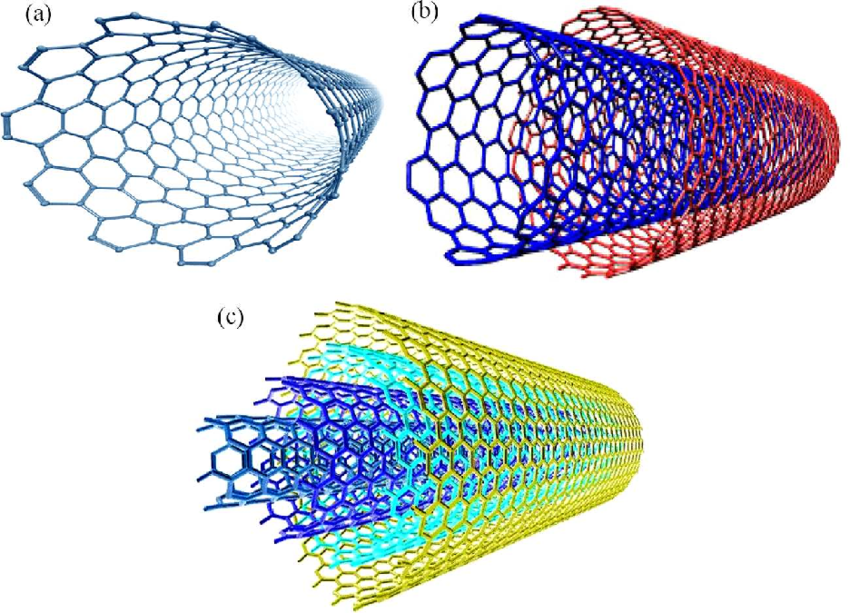
\includegraphics[scale=1]{images/chapter_optical_props/swcnt_mwcnt_rafiq}
	\caption{Schematic diagram showing the crystal structures of (a) a single-wall carbon nanotube (SWCNT), (b) a double-wall carbon nanotube (DWCNT) and (c) a multi-wall carbon nanotube (MWCNT). Reproduced from Ref.\ \cite{rafique2016exploration}.}
	\label{fig:swcnt_mwcnt}
\end{figure}

Due to the similarities between the crystal structures of graphene and SWCNTs, different SWCNT species can be classified using the basis vectors of the graphene lattice \cite{charlier2007electronic}. In fact, the countless ways of rolling up a graphene sheet into a nanotube evince that CNTs can exhibit varying helical geometries and symmetries with respect to their axial direction, as shown in Figure \ref{fig:symmetries}.

\begin{figure}[h]
	\centering
	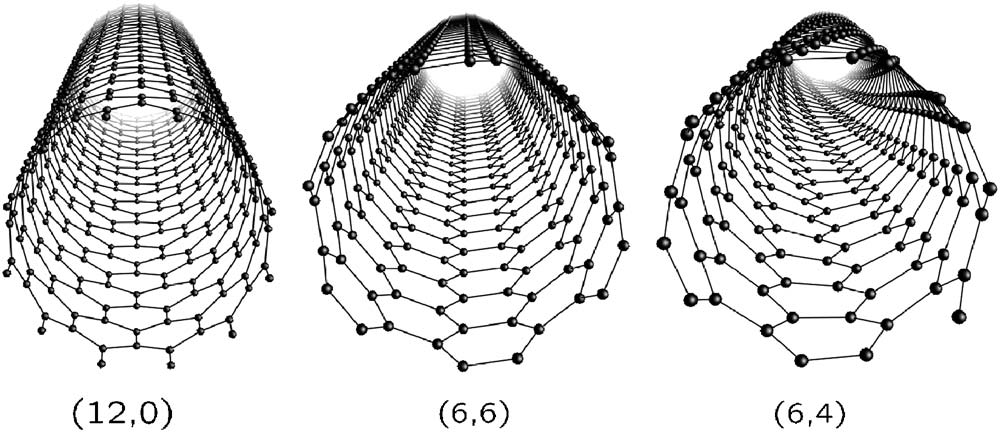
\includegraphics[scale=0.4]{images/chapter_optical_props/nanotube_symmetries_charlier}
	\caption{Crystal structures of (12,0), (6,6) and (6,4) single-wall carbon nanotubes. Reproduced from Ref. \cite{charlier2007electronic}.}
	\label{fig:symmetries}
\end{figure}
These morphological properties dictate the allowed electronic states by asserting boundary conditions on the electron wavefunction along the circumferential direction \cite{charlier2007electronic}. All allowed electronic states exhibit anisotropic features and obey a set of optical selection rules that govern allowed inter-band transitions. Moreover, the effect of strong electron-electron interactions effectively suppress the oscillator strengths associated with optical transitions involving any free-electron continuum states \cite{ando1997excitons}. This behavior distinguishes carbon nanotubes from conventional bulk semiconductors as they typically exhibit relatively weak Coulomb interactions \cite{ando1997excitons}. Finally, the presence of significant electron-electron interactions also means that all optical transitions directly create strongly-correlated quasi-particles known as excitons that dominate the optical properties of SWCNTs.


\section{Definition of the Chiral Vector $\vec{C}_\text{h}$}

Each unique species of carbon nanotubes can be denoted using a set of indices ($n$,$m$). These integers $n$ and $m$ define the chiral vector $\vec{C}_\text{h}$ expressed as
\begin{equation}
	\vec{C}_\text{h} = n \vec{a}_1 + m {\vec{a}_2} \equiv (n,m)
	\label{eq:chiral_vec}
\end{equation}
where $\vec{a}_\text{1} = (\sqrt{3}/2, \text{ }1/2) a$ and $\vec{a}_\text{2} = (\sqrt{3}/2, \text{ }-1/2)a$ represent the primitive lattice vectors of the 2D graphene sheet as shown in Figure \ref{fig:chiral_vectors}. Here, $a = \sqrt{3} a_\text{C-C}$ where $a_\text{C-C} \approx$ \SI{1.44}{\angstrom} denotes the nearest-neighbor distance between carbon atoms in graphene. The vector $\vec{C}_\text{h}$ is also commonly referred to as the roll-up vector as the magnitude $|\vec{C}_\text{h}|$ equals the nanotube circumference $\pi d_\text{t}$, for a given diameter $d_\text{t}$ \cite{nanot2013single}. From this relationship, the diameter $d_\text{t}$ for a nanotube of chirality ($n$, $m$) can be derived as
\begin{equation}
	\begin{split}
		d_\text{t} &= \dfrac{|\vec{C_\text{h}}|}{\pi} \\
		&= \frac{1}{\pi}\sqrt{ n^2 |\vec{a}_1|^2 + 2 n m (\vec{a}_1 \cdot \vec{a}_2) + m^2|\vec{a}_2|^2 }  \\
		&= \frac{1}{\pi}\sqrt{ a^2 n^2 (3/4 + 1/4 )+ 2 a^2 n m (3/4 - 1/4 ) + a^2 m^2 (3/4 + 1/4 ) } \\
		&= \frac{1}{\pi} \sqrt{ a^2 (n^2 + n m + m^2) }\\
		&= \frac{a_\text{C-C}}{\pi}\sqrt{3(n^2 + nm + m^2)}
	\end{split}
\end{equation}
.

\begin{figure}[ht]
	\centering
	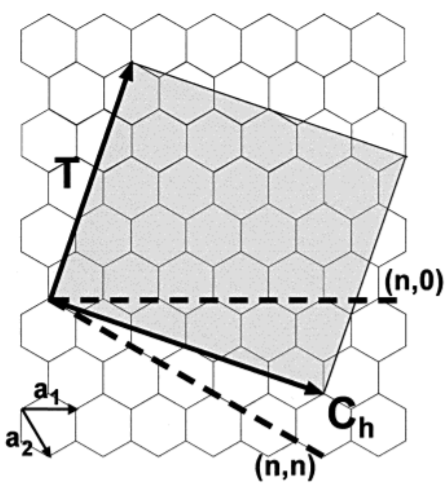
\includegraphics[scale=1]{images/chapter_optical_props/chiral_vectors_sheet.png}
	\caption{Two-dimensional graphene sheet featuring the lattice vectors $\vec{a}_1$ and $\vec{a}_2$ and the chiral vector $\vec{C}_\text{h}$ defined in Equation \eqref{eq:chiral_vec}. The vector $\vec{T}$ points in the axial direction of the carbon nanotube. Furthermore, $(n,n)$ and $(n,0)$ represent limiting cases for $\vec{C}_\text{h}$. Reproduced from Ref. \cite{odom2000structure}.}
	\label{fig:chiral_vectors}
\end{figure}


\section{Optical and Electronic Properties}

\subsection{Electronic Band Structure}

Given the similarities between CNTs and graphene, calculating the electronic band structure of graphene is the first step towards determining that of CNTs. A simple tight-binding model can be used to calculate the band structure of graphene. Such a model includes first nearest-neighbor interactions involving the $\pi$-orbitals of two atomic sites located at positions $\vec{a}_1$ and $\vec{a}_2$ \cite{charlier2007electronic}. Here, $\vec{a}_1$ and $\vec{a}_2$ represent the lattice vectors of graphene. Furthermore, a hopping term $\gamma_0 \approx 2.9$ eV  characterizes the interactions between neighboring $\pi$-orbitals \cite{charlier2007electronic}. The Hamiltonian $\mathcal{H}$ for this simple system is then written as
%
\begin{equation}
	\mathcal{H} = \begin{bmatrix}
	0 & \alpha(k) \\
	\alpha^*(k) & 0
	\end{bmatrix}
\end{equation}
%
where $\alpha(\vec{k}) = (1 + e^{-i \vec{k}\cdot \vec{a}_1} + e^{-i \vec{k}\cdot \vec{a}_2})$ and $\alpha^*(\vec{k})$ refers to the complex conjugate of $\alpha(\vec{k})$ \cite{charlier2007electronic}. In addition, $\vec{k}$ stands for a Bloch vector within the first Brillouin zone. Diagonalizing this matrix yields the energy dispersion
%
\begin{equation}
	E^{\pm} (k_\text{x}, k_\text{y}) = \pm \gamma_0 \sqrt{1 + 4 \cos\dfrac{\sqrt{3}k_\text{x} a}{2}\cos\dfrac{k_\text{y} a}{2} + 4 \cos^2 \dfrac{k_\text{y} a}{2}}
	\label{eq:graphene_band}
\end{equation}
 where $E^-$ and $E^+$ represent the dispersion relations of the valence and conduction bands respectively. The variables $k_\text{x}$ and $k_\text{y}$ denote the $x$ and $y$ components of $\vec{k}$.
%
\begin{figure}[h]
	\centering
	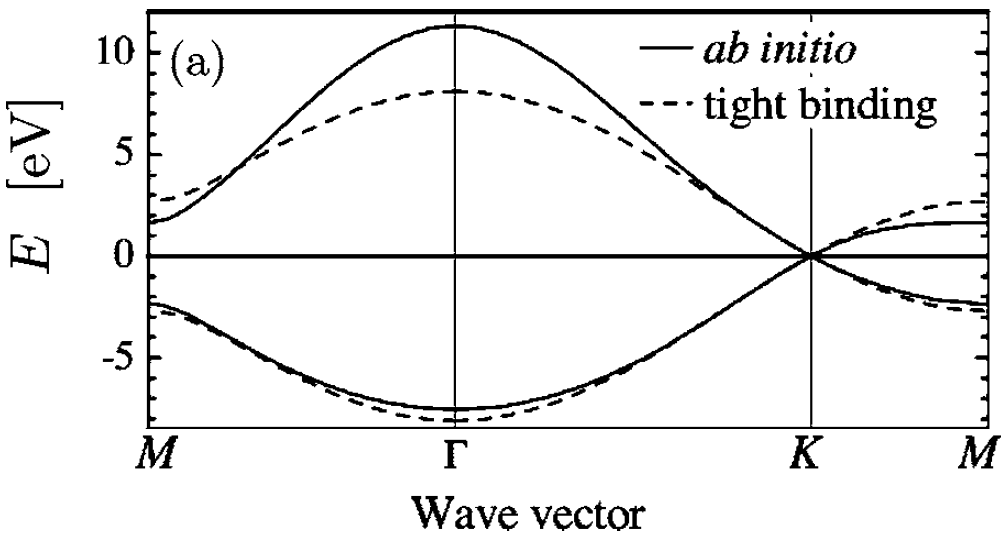
\includegraphics[scale=0.5]{images/chapter_optical_props/graphene_band_charlier}
	\caption{Electronic band structure of graphene determined using a tight-binding model (dashed line) and through ab-initio calculations (solid line). Reproduced and modified from Ref. \cite{reich2002tight}.}
	\label{fig:graphene_band}
\end{figure}

Figure \ref{fig:graphene_band} presents a plot of Equation \eqref{eq:graphene_band} as compared with a band structure calculation using ab-initio methods. The two curves do not predict the same dispersion around the $\Gamma$ point. However, Reich et al.\ note that better agreement is achieved after including interactions between second-nearest and third-nearest neighbor interactions in the original tight-binding model \cite{reich2002tight}. Despite the disagreement between both approaches, they both predict a linear dispersion in the region near the $K$ point in momentum space \cite{charlier2007electronic}. This region of the band structure is commonly referred to as the Dirac cone due to its conical structure shown in Figure \ref{fig:dirac_cone} \cite{charlier2007electronic}. In this region, the energy dispersion approximately becomes
\begin{equation}
	\displaystyle E^{\pm}(\vec{k}) \approx \pm \hbar v_\text{F}|\vec{k}|
\end{equation}
where $\vec{k}$ in this instance is measured with respect to the $K$ point. Furthermore the variable $v_\text{F}$ is the Fermi velocity defined as $v_\text{F} = 3 \gamma_0 a_\text{C-C}/2 \approx 10^6$ m/s. Moreover, both models identify graphene as a zero-gap semiconductor since the valence and conduction bands intersect at the $K$ point \cite{charlier2007electronic}. Without the presence of any dopants, the Fermi level remains exactly at the position where the two bands cross at the $K$ point and the Fermi surface becomes an infinitesimal point.

\begin{figure}[ht]
	\centering
	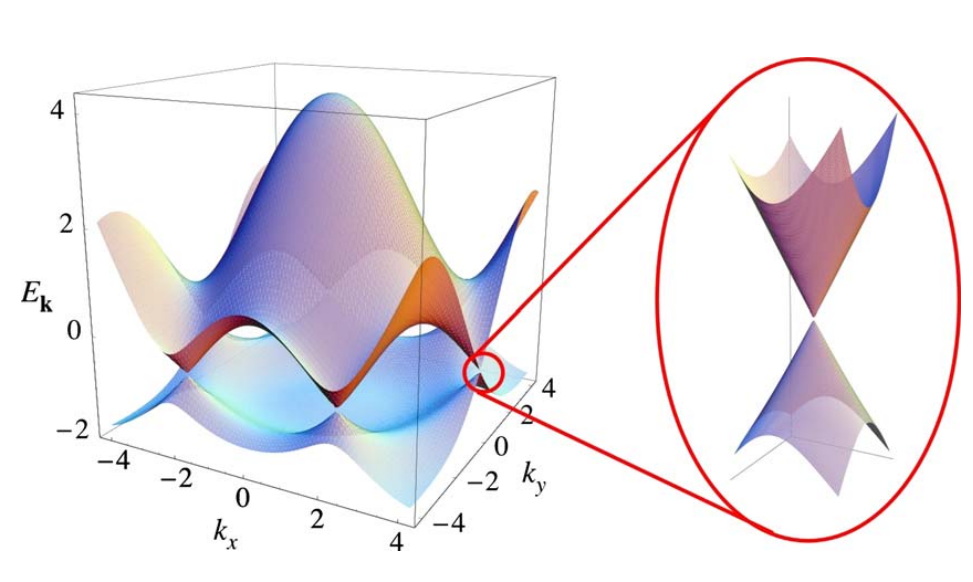
\includegraphics[scale=0.4]{images/chapter_optical_props/dirac_cone}
	\caption{Electronic band structure of graphene with energy in units of $\gamma_0$. Close to the $K$ point, the dispersion becomes approximately linear in a region known as the Dirac cone. Reproduced from Ref.\ \cite{neto2009electronic}.}
	\label{fig:dirac_cone}
\end{figure}


\subsection{Chiralities of Semiconducting and Metallic Nanotubes}

\begin{figure}[ht]
	\centering
	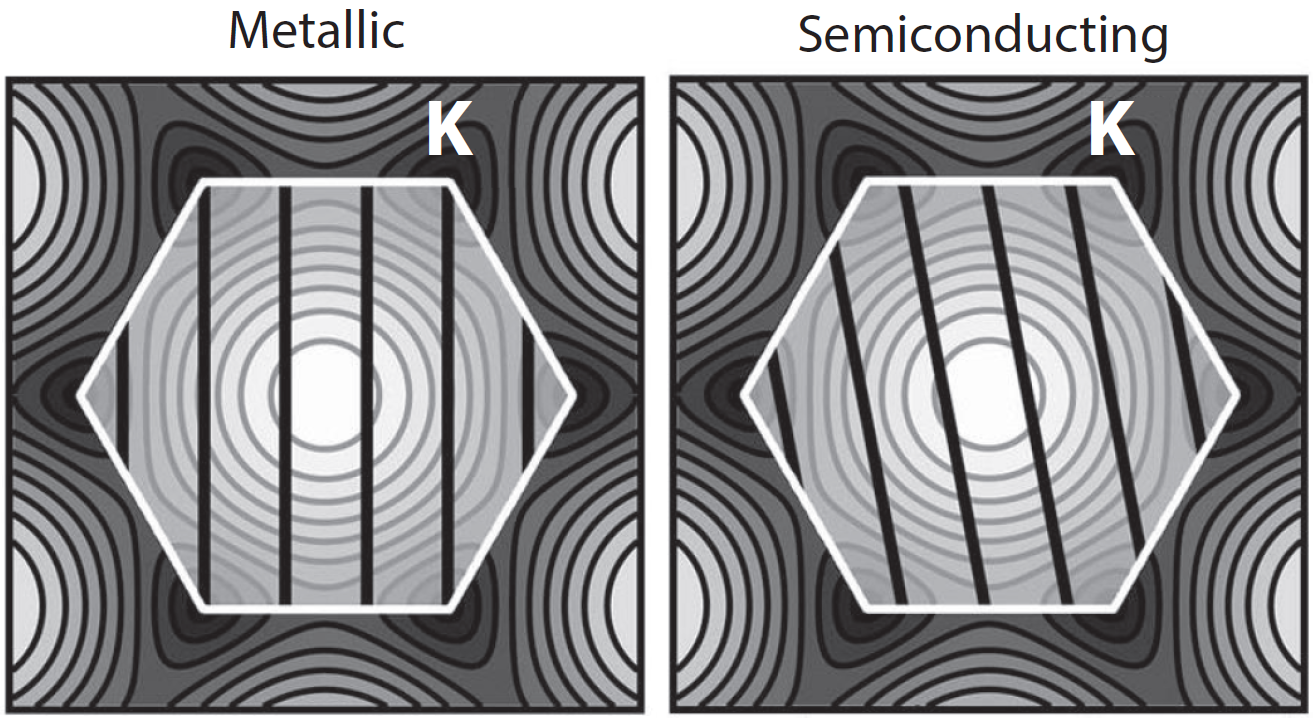
\includegraphics[scale=0.35]{images/chapter_optical_props/metal_semi_amori}
	\caption{The image shows the first Brillouin zone of graphene (white hexagon) superimposed on a countour map of the electronic band structure of graphene. The Dirac point sits at the K point. Allowed values of $\vec{k}$ according to the quantization condition defined in Equation \eqref{eq:quantization_cond} are drawn over the Brillouin zone as thick, black, vertical lines. For metallic nanotubes, the electronic states located at the Dirac point are allowed. Whereas, the band structures of semiconducting nanotubes do not include a Dirac point. Reproduced from Ref.\ \cite{amori2018excitons}.}
	\label{fig:k_quant}
\end{figure}

In conjunction with the band structure of graphene, the zone-folding approximation yields the band structure of CNTs. The zone-folding method asserts that the periodic boundary conditions along the circumferential direction of CNTs dictate the quantization of the allowed $\vec{k}$ vectors in the electronic band structure \cite{charlier2007electronic}. This condition applied to the electron wavefunction $\Psi(\vec{r})$ is expressed as
\begin{equation}
\Psi_{\vec{k}}(\vec{r} + \vec{C}_\text{h}) = e^{i \vec{k} \cdot \vec{C}_\text{h}} \Psi_{\vec{k}}(\vec{r}) = \Psi_{\vec{k}}(\vec{r}),
\label{eq:boundary_cond}
\end{equation}
where $\vec{r}$ and $\vec{k}$ respectively define vectors in real and reciprocal space on the surface of the CNT \cite{charlier2007electronic}. Furthermore, $\vec{C}_\text{h}$ represents the chiral vector defined in Equation \eqref{eq:chiral_vec}. This condition gives the quantization of $\vec{k}$ which can be written as
\begin{equation}
	\vec{k} \cdot \vec{C}_h = 2\pi n
	\label{eq:quantization_cond}
\end{equation}
for a given integer $n$. Equation \eqref{eq:quantization_cond} reveals that the symmetry of the CNT given by the chirality $\vec{C}_\text{h} \equiv (n,m)$ determines the band structure. Figure \ref{fig:k_quant} illustrates this. Depending on the chirality of the nanotube, the Dirac point located at the K point may or may not be included the nanotube's bandstructure. This may determine whether or not the nanotube has a finite band gap energy.

In addition, the variable $\nu$ defined as
%
\begin{equation}
\label{eq:nu_cnt}
\nu \equiv (n-m) \mathrm{\hspace{1.5mm} mod \hspace{1.5mm}} 3,
\end{equation}
%
is also used to classify the two different band structures that can occur.
%
\begin{figure}[h]
	\centering
	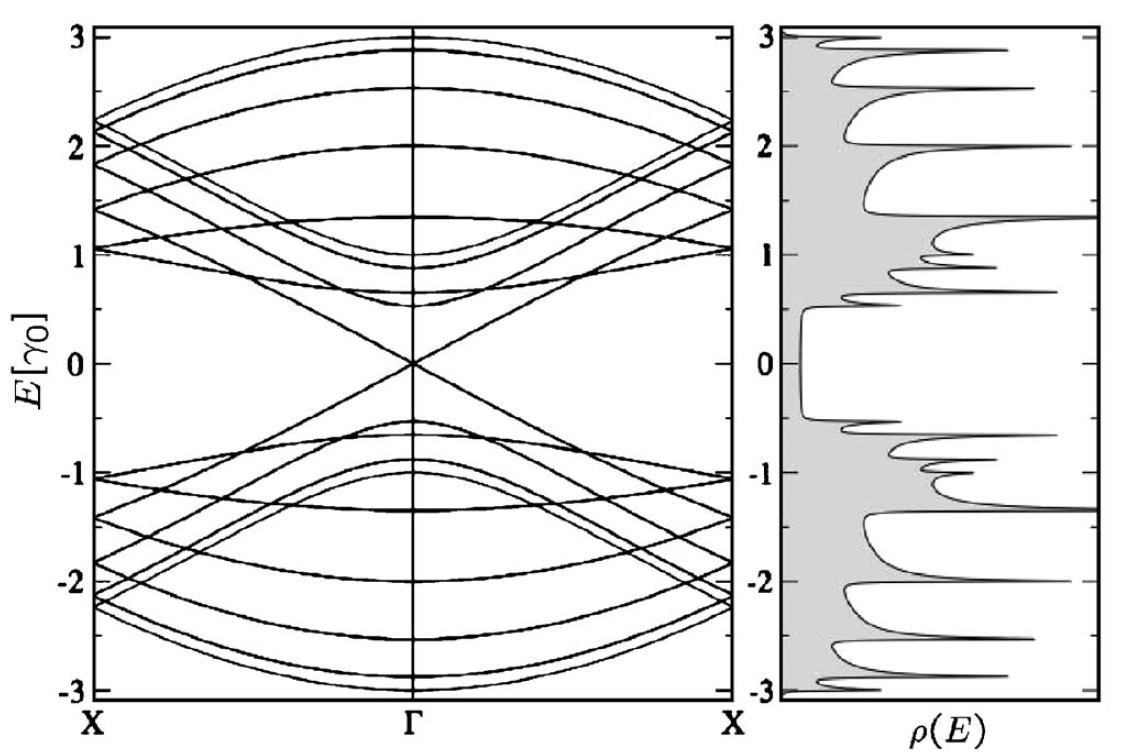
\includegraphics[scale=0.3]{images/chapter_optical_props/nine_zero_band_charlier}
	\caption{Band structure and density of states for a (9,0) carbon nanotube derived using the zone-folding scheme. These are plotted in units of $\gamma_0 \approx 2.9$, the tight-binding hopping energy between first nearest-neighbors. Reproduced from Ref.\ \cite{charlier2007electronic}.}
	\label{fig:nine_zero_cnt}
\end{figure}
%
In the case where $\nu = 0 $, the band structure contains a Dirac point along with additional sub-bands within the valence and conduction bands, as presented in Figure \ref{fig:nine_zero_cnt}. CNTs that satisfy this condition include $(n,n)$ carbon nanotubes, also commonly referred to as ``armchair'' nanotubes, that constitute the set of all metallic (gapless) nanotubes \cite{nanot2012optoelectronic}. Furthermore, $(n,m)$ nanotubes where $n-m = 3j$ ($j > 0$) also satisfy this $\nu = 0$ condition. However, these non-armchair nanotubes ($n\neq m$) exhibit curvature-induced band gaps and can behave as narrow-gap semiconductors ($\sim1 - 100$ meV band gap energy) \cite{nanot2012optoelectronic}. This is caused by local deformations of the nanotube surface that enhance electron transfer in the circumferential direction   \cite{hamada1992new, kane1997size}. These deformations cause the $\pi$-orbitals, which are typically oriented normal to the tubule surface and are parallel to each other, to instead become angled. As a result, this enhances the hopping term between a subset of neighboring $\pi$-orbitals, thereby opening an energy gap in the band structure.

When $\nu= \pm 1$, the band structure corresponds to that of a medium-gap semiconductor ($\sim0.5 - 1$ eV band gap energy) \cite{nanot2012optoelectronic}. This band structure excludes the presence of a Dirac point as shown in Figure \ref{fig:ten_zero_cnt}  \cite{charlier2007electronic}.

%\begin{figure}[h]
%	\centering
%	\begin{subfigure}{0.45\textwidth}
%		\centering
%		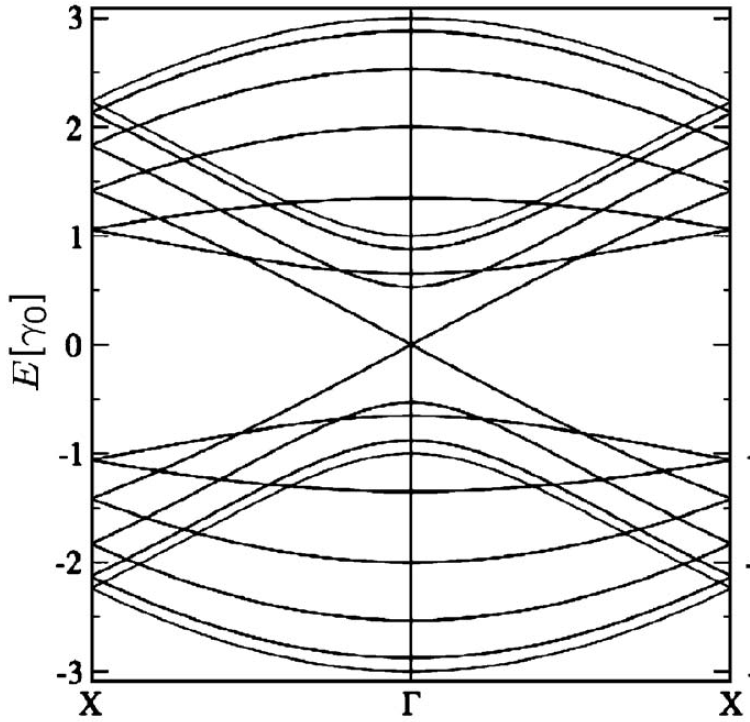
\includegraphics[scale=0.36]{images/chapter_optical_props/nine_zero_band_charlier_2}
%		\caption{Metallic}
%	\end{subfigure}
%	\qquad
%	\begin{subfigure}{0.45\textwidth}
%		\centering
%		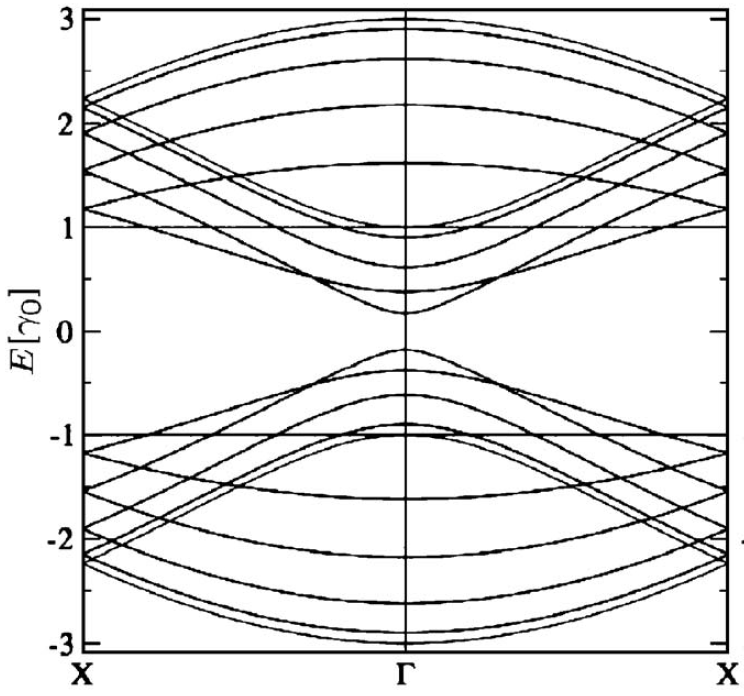
\includegraphics[scale=0.38]{images/chapter_optical_props/ten_zero_band_charlier_2}
%		\caption{Metallic}
%	\end{subfigure}
%	\caption{Reproduced and modified from Ref \cite{charlier2007electronic}.}
%\end{figure}


\begin{figure}[ht]
	\centering
	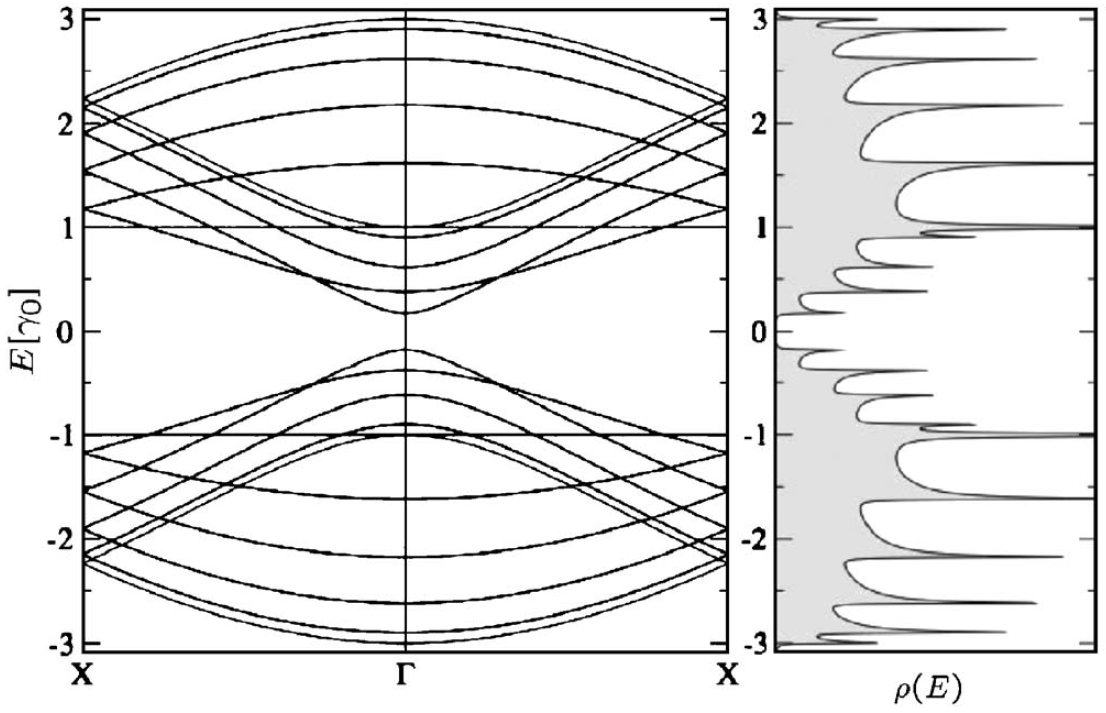
\includegraphics[scale=0.33]{images/chapter_optical_props/ten_zero_band_charlier}
	\caption{Band structure and density of states for a (10,0) carbon nanotube derived using the zone-folding scheme. These are plotted in units of $\gamma_0 \approx 2.9$ eV which represents the tight-binding hopping energy between first nearest-neighbors. Reproduced from \cite{charlier2007electronic}.}
	\label{fig:ten_zero_cnt}
\end{figure}


\subsection{Optical Selection Rules}
\label{section:selection_rules}

Selection rules dictate the set of dipole-allowed optical transitions that can occur. Such optical processes depend upon the conservation of, energy, momentum, and parity \cite{bovzovic2000optical}. Figure \ref{fig:allowed_optical_transitions} shows an energy diagram of all dipole-allowed transitions for metallic ($\nu = 0$) and semiconducting CNTs ($\nu=\pm 1$) for cases when polarization of the photon is parallel ($\Delta n = 0 $) or perpendicular ($\Delta n = \pm 1 $) to the nanotube's long axis. Here, each sub-band is indexed by the parameter $n$. The notation E$_{ij}$ is also often used to denote an inter-band transition between the valence sub-band of index $i$ and the conduction sub-band of index $j$ \cite{weismanKonoBook}. According to the diagram, the transitions such as $E_{11}$, $E_{22}$, and $E_{33}$ can occur in the case where light is polarized parallel to the nanotube's long axis, whereas transitions such as $E_{12}$, $E_{21}$, and $E_{23}$ can occur in the perpendicular case. Finally, it is also assumed here that incident photons travel towards the CNT surface at normal incidence.

\begin{figure}[ht]
	\centering
	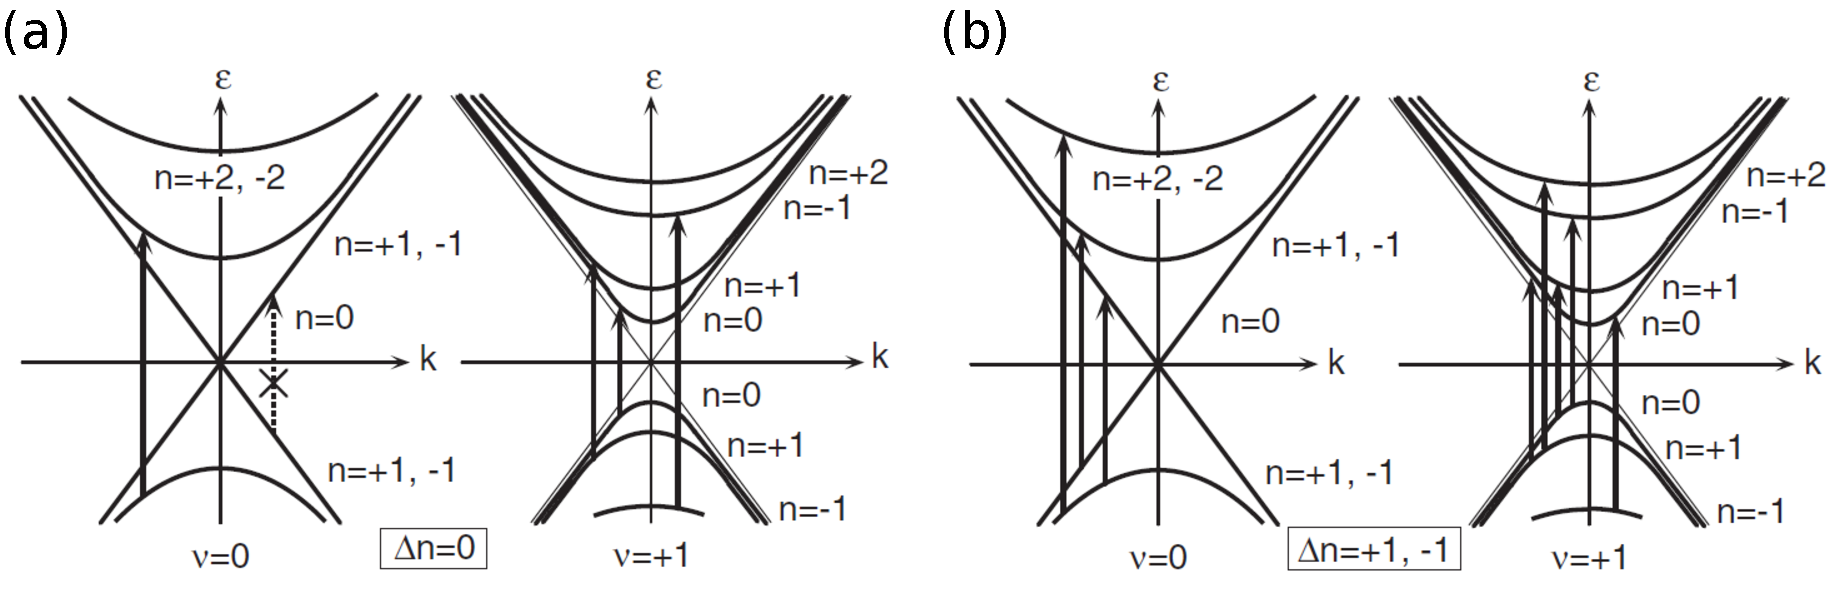
\includegraphics[scale= 0.52]{images/chapter_optical_props/selection_rules_combined}
	\caption{Optical selection rules for metallic ($\nu = 0 $) and semiconducting nanotubes ($\nu = \pm 1$). These include cases where the incident light is polarized parallel to the nanotube axis (a) or polarized perpendicular to the nanotube axis (b). Reproduced from Ref.\ \cite{ando2005theory}}
	\label{fig:allowed_optical_transitions}
\end{figure}

 One method of elucidating these selection rules involves the use of symmetry groups tied to the nanotube crystal structure to determine the linear and angular momentum of each distinct electron state \cite{bovzovic2000optical}. As shown in Figure \ref{fig:cnt_symmetries} , two relevant symmetries of carbon nanotubes include the symmetry about the nanotube axis denoted as $\sigma_\text{v}$, as well as the symmetry with respect to the the radial direction represented as $\sigma_\text{h}$ \cite{bovzovic2000optical}. Moreover, the symmetry groups $\sigma_\text{v}$ and $\sigma_\text{h}$ can each be associated with two distinct quantum numbers respectively. These include $k$, the momentum along the nanotube axis related to the translation symmetry of the nanotube as well as $n$, the z-component of the angular momentum associated with nanotube's rotational symmetry.

 \begin{figure}[ht]
 	\centering
 	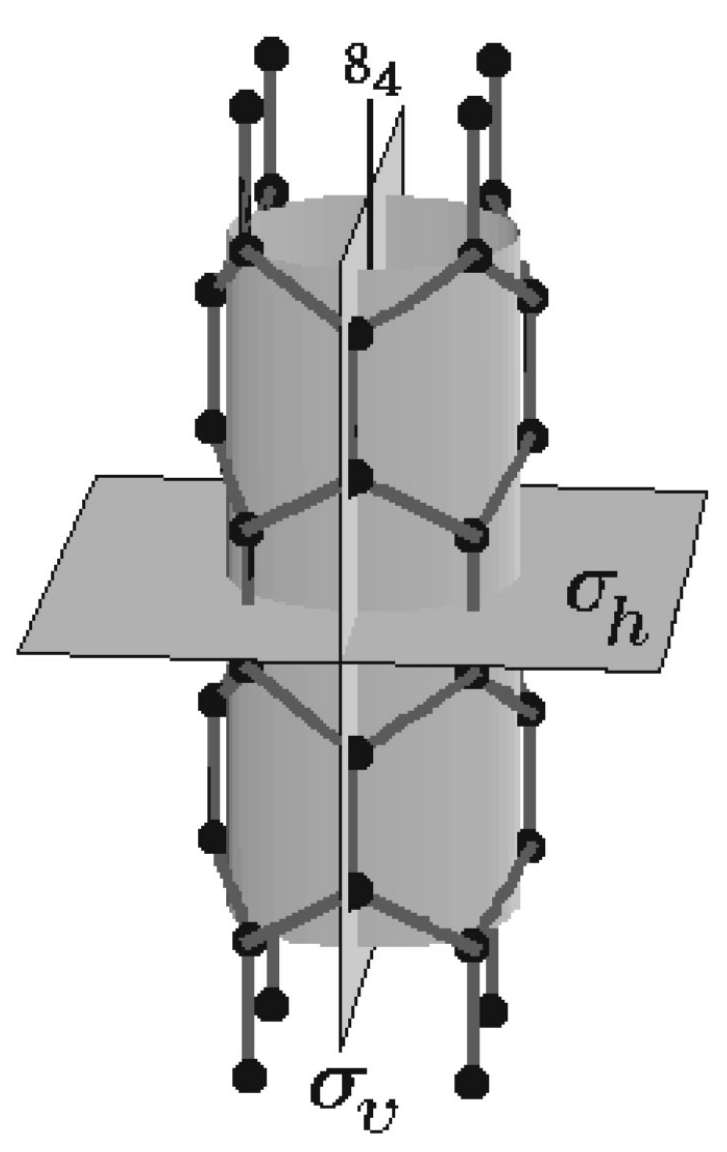
\includegraphics[scale=0.15]{images/chapter_optical_props/cnt_symmetry_bozovic}
 	\caption{(a) Crystal structure of a (4,0) carbon nanotube with symmetry planes $\sigma_\text{h}$ and $\sigma_\text{v}$.}
 	\label{fig:cnt_symmetries}
 \end{figure}

 Light has a negligible linear momentum which imposes the condition that transitions can only occur between two states such that the difference in the linear momenta of these two states $\Delta k \approx 0 $ \cite{bovzovic2000optical}. However, an incident photon can carry a finite angular momentum depending on its polarization with respect to the nanotube axis. Correspondingly, each subband can indeed be indexed according to their angular momentum. Incident light that is linearly polarized perpendicular to nanotube axial direction has angular momentum $n = \pm 1$. More specifically, right-handed, circular polarization has $n = 1$ whereas, left-handed circular polarization has $n = -1$. In this geometry, optical transitions where the change between the initial and final angular momentum $\Delta n = \pm 1$ can occur.

The symmetry planes can also be used to described the parity conservation of each optical transition. For optical transitions where $\Delta n = 0$, parity becomes conserved about the $\sigma_\text{v}$ plane and reversed about the  $\sigma_\text{h}$. For the optical transitions where $\Delta n = \pm 1$, parity becomes conserved about the $\sigma_\text{h}$ plane and reversed with respect to the $\sigma_\text{v}$ plane.

%These results yield enough information to deduce the set of dipole-allowed transitions. In the case where incident light is polarized parallel to the nanotube axis, transitions that satisfy the condition $\Delta m = 0$ can occur \cite{bovzovic2000optical}. One interpretation of this is that optical transitions can only occur between bands with the same band index. When light is polarized perpendicular to the nanotube axis, this now permits optical transitions where $\Delta m = \pm 1$ \cite{bovzovic2000optical}. In other words, optical transitions can occur between bands whose band indices differ by one \cite{weismanKonoBook}.


%For light polarized parallel to z-direction, parity with respect to $\sigma_\text{v}$ is preserved whereas parity with repsect to $\sigma_\text{h}$ is reversed. In other words, transitions can occur between bands that have the same parity with respect to $\sigma_\text{v}$. However, one of the bands involved in optical transition must have event parity with respect to $\sigma_\text{h}$ whilst the other band has odd parity with respect to $\sigma_\text{h}$.

%In the case of light polarized perpendicular to the z-direction, parity with respect to $\sigma_\text{v}$ is reversed whereas parity with respect to $\sigma_\text{h}$ is preserved.

%\begin{figure}[H]
%	\centering
%	\begin{subfigure}{\textwidth}
%		\centering
%		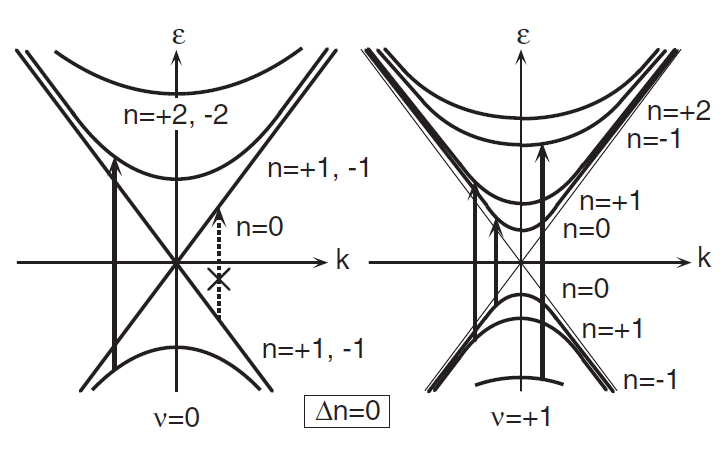
\includegraphics[scale=0.65]{images/chapter_optical_props/selection_rules_1.png}
%		\caption{Selection Rules for light polarized parallel to the axial direction of carbon nanotubes. In the $\nu=0$ case, transitions within the Dirac cone are forbidden.}
%	\end{subfigure}
%	\begin{subfigure}{\textwidth}
%		\centering
%		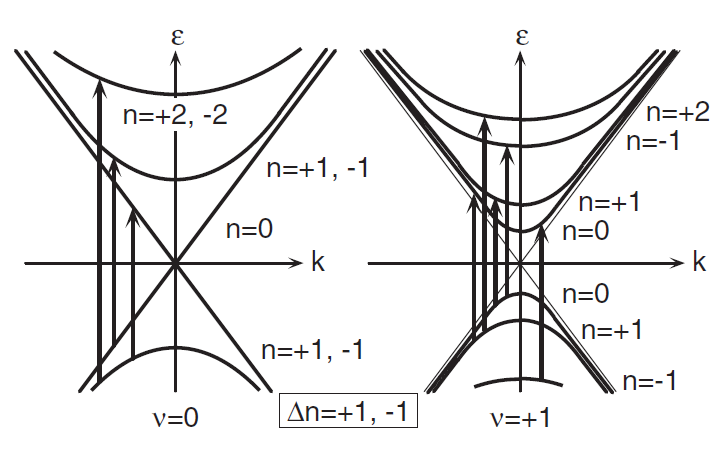
\includegraphics[scale=0.65]{images/chapter_optical_props/selection_rules_2.png}
%		\caption{Selection Rules for light polarized perpendicular to the axial direction of carbon nanotubes.}
%	\end{subfigure}
%	\caption{Optical selection rules for metallic and narrow-gap semiconducting nanotubes ($\nu = 0 $) as well as medium-gap semiconducting nanotubes ($\nu = \pm 1$) . Reproduced from Ref.\ \cite{ando2005theory}.}
%	\label{fig:selection_rules}
%\end{figure}



\section{Excitons in SWCNTs}

\subsection{Supression of Optical Transitions Involving the Free-Electron Continuum}

One peculiar feature of 1D materials, as compared with 2D or 3D systems, is the relatively low interband absorption associated with the creation of free electron-hole pairs \cite{ogawa1991interband}. A key aspect of this phenomenon involves excitons which represent hydrogen-like quasi-particles composed of a negatively-charged electron bound to a positively-charged hole via Coulomb interactions \cite{Ashcroft, kira2011semiconductor}. For an ideal 1D material, theory predicts that excitons will have an infinite binding energy \cite{loudon1959one, elliott1959theory}. This alone foreshadows the profound effect of excitons on the optical properties of 1D systems.

In describing how excitons affect the optical absorption of 1D materials, Ogawa \textit{et al.} (1991) introduced the concept of the Sommerfeld factor, defined as the ratio between the optical absorption of the unbound exciton continuum ($K_\text{exciton}$) to the that of the free-electron continuum ($K_\text{e-h}$) above the band gap energy $E_g$. This can be expressed as
\begin{equation}
	S_\text{a} (\omega) = \frac{K_\text{exciton}(\omega)}{K_\text{e-h}(\omega)},
\end{equation}
where $\hbar \omega > E_\text{g}$. As an aside, this concept was originally developed by Arnold Sommerfeld to explain the enhancement of electron-positron annihilation cross-section due to the Coulomb interaction between the two charged particles \cite{sommerfeld1931beugung}. In the context of condensed matter systems, the Sommerfeld factor shows how the Coulomb interactions between electrons and holes can either enhance or reduce the optical absorption of the free electron continuum states \cite{ogawa1991interband}.

\begin{figure}[ht]
	\centering
	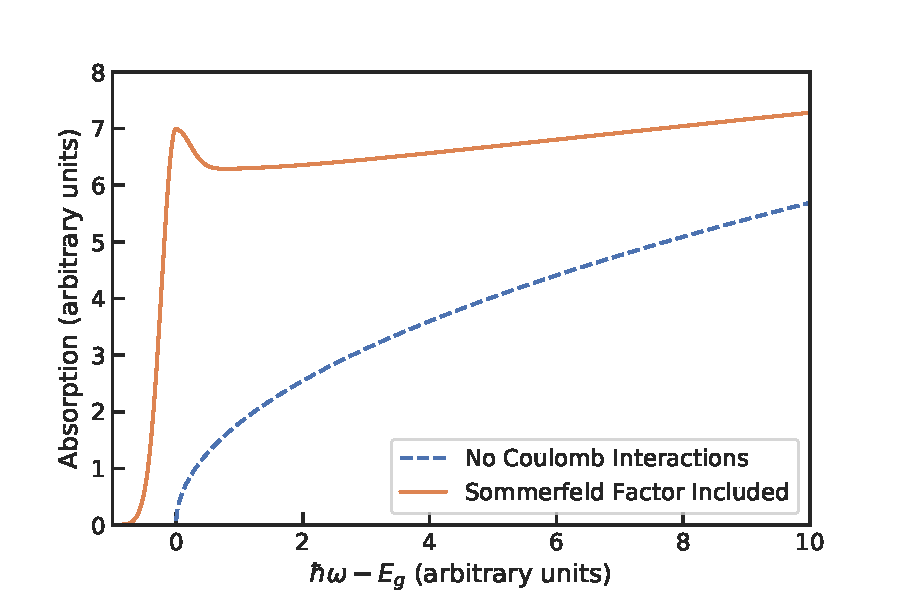
\includegraphics[scale=0.8]{images/chapter_optical_props/Sommerfeld_Plot/coulomb_enhancement}
	\caption{Plot of optical absorption spectrum demonstrating the effect of Coulomb interactions on the oscillator strength of interband transitions in a 3D system. With no Coulomb interactions the absorption varies as $\sqrt{\hbar\omega - E_\text{g}}$ from the standard 3D free-electron gas model \cite{Ashcroft}. After including Coulomb interactions, an exciton peak appears near the band edge and the interband absorption becomes enhanced.}
	\label{fig:coulomb_enhancement_3d}
\end{figure}

For 2D or 3D systems, $S_\text{a}$ always remains above unity, suggesting that Coulomb interactions enhance interband absorption in these scenarios \cite{ogawa1991interband}. In the case of 3D systems, the Sommerfeld factor is given as
\begin{equation}
	S_\text{a}^\text{3D}(\omega) = \frac{\pi \alpha \exp(\pi \alpha)}{\sinh(\pi \alpha)}
\end{equation}
for dipole-allowed transitions \cite{elliott1957intensity}. Here, $\alpha \propto 1/\sqrt{\hbar\omega - E_\text{g}}$. This result is demonstrated in Figure \ref{fig:coulomb_enhancement_3d}. Coulomb interactions not only result in an exciton peak near the band edge but also enhance optical absorption above the band gap.


However, for 1D systems, $S_\text{a}^\text{1D}$ always remains below unity for energies above the the band gap \cite{ogawa1991interband}. Figure \ref{fig:coulomb_enhancement_1d} shows the effect of the 1D Sommerfeld factor on the optical absorption of a 1D material. Unlike the 3D case, the exact expression for $S_\text{a}^\text{1D}$ is more complicated as it involves a gamma function along with two basis solutions of a confluent hypergeometric eqquation \cite{ogawa1991optical}. In general however, $S_\text{a}^\text{1D} = 0$ at the band edge \cite{ogawa1991optical} and monotonically increases \cite{ogawa1991optical}. This plot therefore uses a tanh function for simplicity to approximate these features of $S_\text{a}^\text{1D}(\omega)$. The plot shows the presence of van Hove singularities when ignoring the effect of Coulomb interactions. After accounting for these interactions, the Sommerfeld factor indicates a suppression of interband optical absorption. Most of the oscillator strength of the optical absorption instead resides with lowest-lying exciton peak.


\begin{figure}[ht]
	\centering
	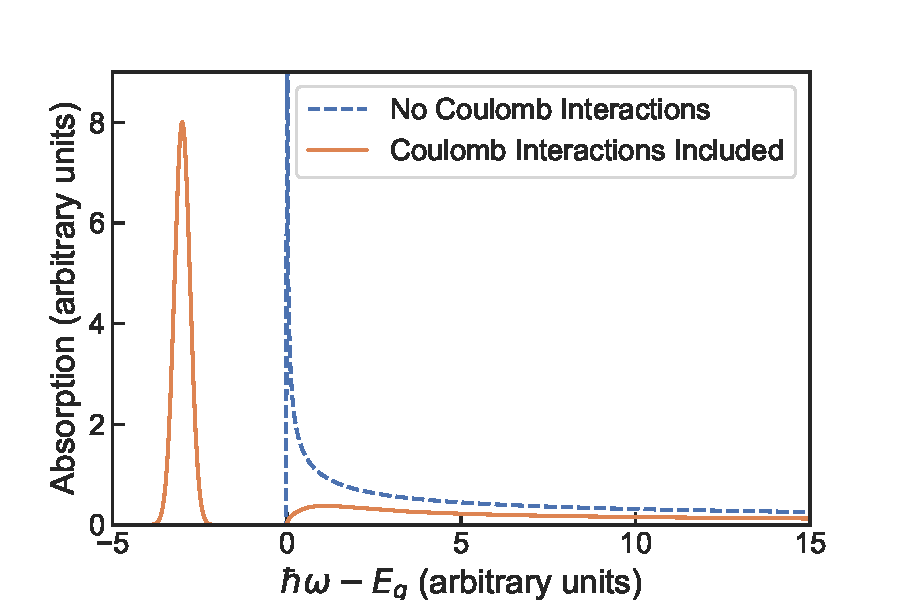
\includegraphics[scale=0.8]{images/chapter_optical_props/Sommerfeld_Plot/coulomb_enhancement_1d}
	\caption{Plot of optical absorption spectrum demonstrating the effect of Coulomb interactions on the oscillator strength of interband transitions in a 1D system. In this case, the Sommerfeld factor is approximated as a tanh function for simplicity. With no Coulomb interactions the absorption varies as $1/\sqrt{\hbar\omega - E_\text{g}}$ from the 1D free-electron gas model \cite{Ashcroft}. After including Coulomb interactions, an exciton peak appears below the band edge and the interband absorption for the free electron continuum becomes supressed. }
	\label{fig:coulomb_enhancement_1d}
\end{figure}


%\begin{figure}[ht]
%	\centering
%	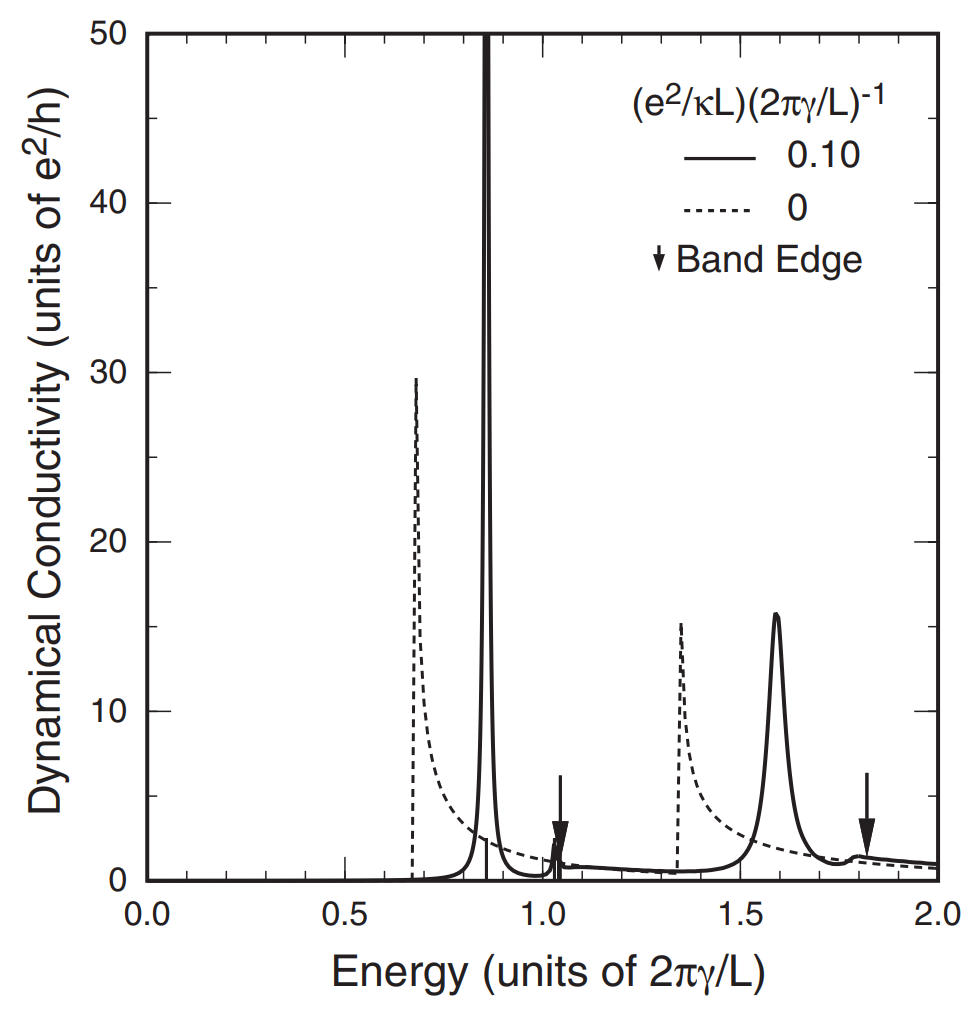
\includegraphics[scale=0.3]{images/chapter_optical_props/ando_suppression}
%	\caption{Optical absorption spectrum of a semiconducting nanotube with (solid line) and without (dashed line) the effect of Coulomb interactions. Arrows mark the band edge positions of free electron continua. Reproduced and modified from Ref.\ \cite{ando2005theory}.}
%	\label{fig:ando_suppression}
%\end{figure}

Exciton energy levels and wavefunctions are largely influenced by the effect of long-range Coulomb interactions \cite{ando2006effects}. Moreover, the effective strength of Coulomb interactions $S_\text{e-e}$ can be expressed as
%
\begin{equation}
	S_\text{e-e} \equiv \dfrac{e^2 \kappa / L}{2 \pi \gamma / L},
\end{equation}
%
where $e^2 /\kappa L$ and $2 \pi \gamma / L$ account for the characteristic energy scales associated with Coulomb interactions and the kinetic energy of electrons respectively \cite{ando2005theory}. Here, $e$ defines the charge of an electron, $\gamma$ represents a band parameter, $L$ indicates the nanotube circumference $|\vec{C}_\text{h}|$, and $\kappa$ denotes the static dielectric constant used to account for screening effects.

Figure \ref{fig:coulomb_shift} shows how the energy levels of the fundamental and second band gaps alongside the exciton bound states changes with the strength of Coulomb interaction. In fact, the band edges of free-electron continua also blue-shift as a result of long-range electron-electron interactions when compared with the case where there are no electron-electron interactions \cite{ando1997excitons}. This relative shift of the band edge also increases as $S_{e-e}$ increases \cite{ando2005theory}. These effects however are more significant for the fundamental band gap than for the second band gap \cite{ando2005theory}. Correspondingly, the binding energy of excitons also increase as the effect of electron-electron interactions become more significant although, the energy level positions for excitons do not change as much as they do for free electrons \cite{ando2005theory}.

\begin{figure}[ht]
	\centering
	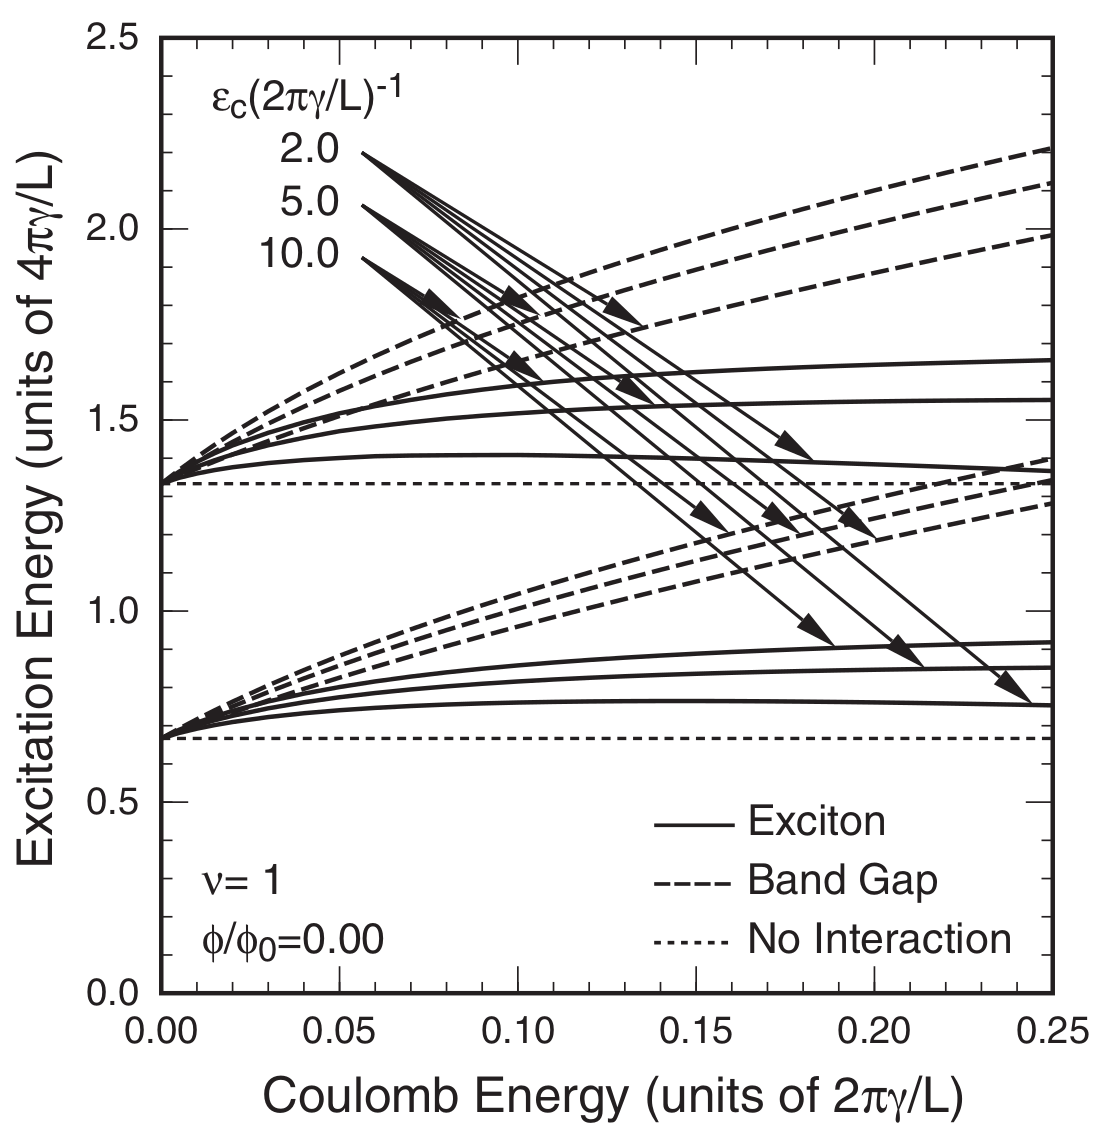
\includegraphics[scale=0.25]{images/chapter_optical_props/coulomb_shift_ando}
	\caption{Calculated energy levels of fundamental and second band gaps (dashed lines) as well as exciton absorption energy as a function of the effective Coulomb energy $(e^2 \kappa / L) (2 \pi \gamma / L)$. Each curve corresponds to a different cutoff energy $\varepsilon_\text{c}$ that limits the range of Coulomb interactions in the model. Reproduced from Ref.\ \cite{ando2005theory}.}
	\label{fig:coulomb_shift}
\end{figure}

\clearpage

\subsection{Exciton Binding Energies}

In essence, the exciton binding energy characterizes the strength of the Coulomb interaction between an electron and its corresponding hole \cite{valkunas2006exciton}. On one hand, if the exciton binding energy is smaller than the thermal energy $k_\text{B} T$, defined using the Boltzmann constant $k_\text{B}$ and a given temperature $T$, then this Coulomb interaction becomes negligible \cite{valkunas2006exciton}. This causes electrons and holes to behave independently of each other. On the other hand, if the binding energy is much higher than the thermal energy, then electrons and holes tend to form stable, charge-neutral excitons \cite{valkunas2006exciton}.

\begin{figure}[ht]
	\centering
	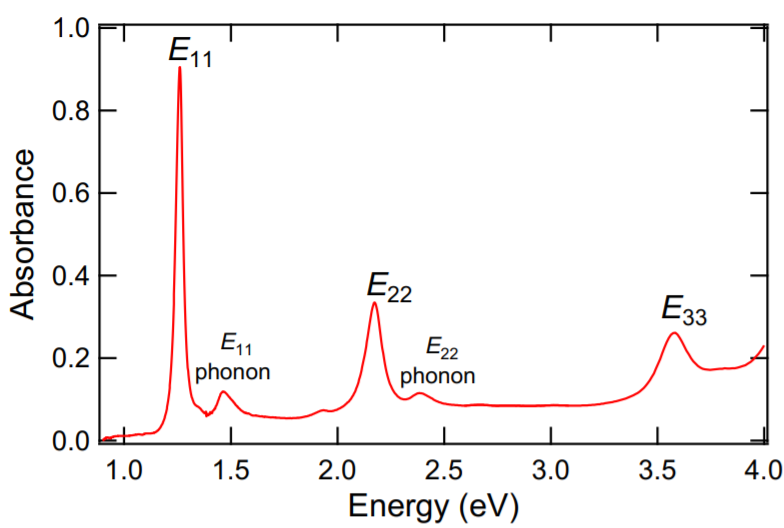
\includegraphics[scale=0.6]{images/chapter_intro/abs_fumiya}
	\caption{Absorbance spectrum of a (6,5) carbon nanotube sample at room temperature. The peaks at 983 and 570 nm correspond to the $E_{11}$ and $E_{22}$ of (6,5) carbon nanotubes. The $E_{12}$ transition of (6,5) nanotubes can also be observed at 650 nm. Reproduced from Ref.\ \cite{katsutani2019direct}. }
	\label{fig:cnt_abs_fumiya}
\end{figure}

The binding energies of excitons in CNTs tend to be on the order of hundreds of meV \cite{wang2005optical}. For instance, the excitons of (6,5) nanotubes have a binding energy of roughly 400 meV \cite{wang2005optical}. At room temperature, $k_\text{B} T \approx$ 26 meV, meaning that the energy scale associated with thermal fluctuations falls short of the exciton binding energies in CNTs. Thus, excitons of CNTs are quite stable at room temperature. Figure \ref{fig:cnt_abs_fumiya} illustrates this effect as the room-temperature absorbance spectrum of a (6,5) sample exhibits well-defined, excitonic resonances.

Two-photon absorption measurements provided experimental evidence of large exciton binding energies in CNTs, generally on the order of hundreds of meV \cite{maultzsch2005exciton, wang2005optical}. Excitons possess a set of Rydberg states, analogous to the hydrogen atom, that can include even parity states such as 1$s$, 2$s$, and 3$s$ as well as odd parity states such as 2$p$, 3$p$, and so on \cite{wang2005optical}. On one hand, optical selection rules establish that one-photon excitations access excitons whose wavefunctions have even parity ($s$-symmtery) \cite{wang2005optical}. On the other hand, two-photon excitation creates excitons whose wavefunctions exhibit odd parity ($p$-symmetry) \cite{wang2005optical}.

\begin{figure}[ht]
	\centering
	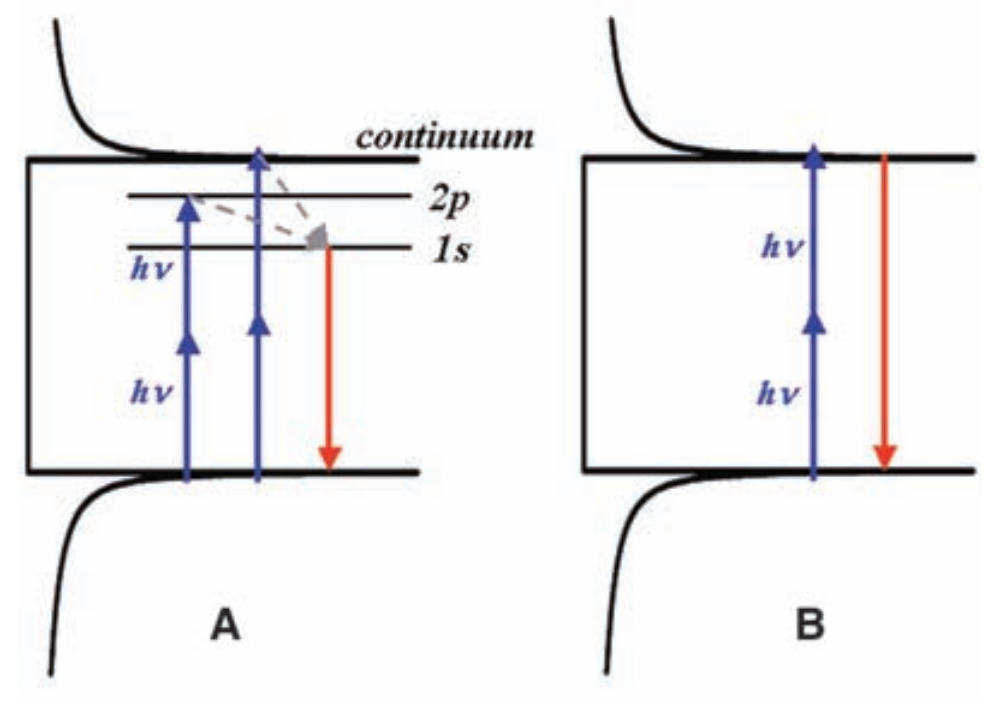
\includegraphics[scale=0.3]{images/chapter_optical_props/cnt_two_photon}
	\caption{ Two-photon absorption in the presence of electron continuum states (A) with and (B) without low lying exciton states within the band gap. When excitonic states are present, two-photon absorption can excite free electron-hole pairs or 2$p$ excitons which then decay to $1s$ excitons before optical recombination occurs. Without exciton states, photoluminescence occurs at the band gap energy from optical recombination of free electrons. Reproduced from Ref.\ \cite{wang2005optical}. }
	\label{fig:cnt_two_photon}
\end{figure}

%For light polarized parallel to the nanotube axial direction, one-photon absorption processes require parities of the initial and final state to be opposite of each other. In contrast, two-photon absorption processes require both the initial and final state to have the same parity.


\begin{figure}[ht]
	\centering
	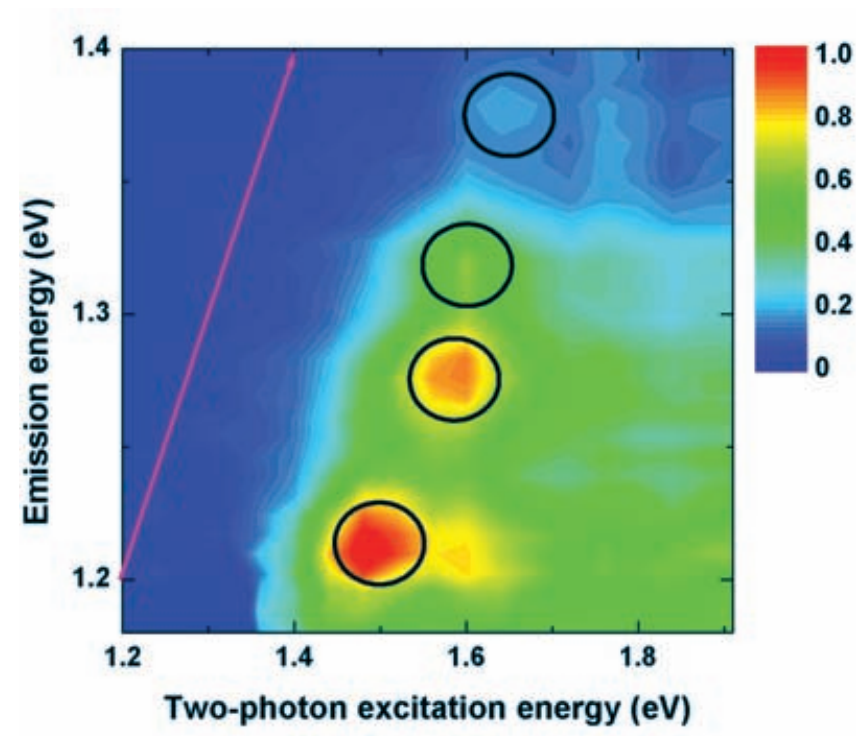
\includegraphics[scale=0.3]{images/chapter_optical_props/two_photon_wang}
	\caption{Contour plot showing emission of various SWCNTs after two-photon excitation. With increasing emission photon energy, fluorescence peaks associated with (7,5), (6,5), (8,3), and (9,1) respectively (black circles). Light emission only occurs when the two-photon exciation energy exceeds that of the emission energy. The solid line on the left-hand side shows the position where emission would occur if the tight-binding were correct. Here, the emission energy would be equal to that of the two-photon excitation energy. Reproduced from Ref.\ \cite{wang2005optical}.}
	\label{fig:cnt_two_photon_emission}
\end{figure}

In practice, this means that one-photon absorption can access the 1$s$ exciton resonance and that two-photon absorption can access excited states above the 1$s$ exciton state, as shown in Figure \ref{fig:cnt_two_photon}. Although other excited states can be accessed, these tend to have almost negligible oscillator strengths \cite{wang2005optical}. Hence, two-photon excitation can create $2p$ excitons which then relax to the $1s$ exciton state before optical recombination occurs at the $1s$ exciton energy.

If there were no exciton states, the optical emission would be most efficient if the two-photon excitation energy (2$\hbar \omega$) were exactly equal to the band gap energy due to the density of states associated with the van Hove singularity. The photon energy of the emission would also be equal to 2$\hbar \omega$. Figure \ref{fig:cnt_two_photon_emission} shows that optical emission instead occurs when the two-photon excitation energy is higher than photon energy of emission, which provides a direct estimate of the 1$s$ - 2$p$ energy separation..

Unlike carbon nanotubes, conventional semiconductors such as GaAs only exhibit excitons with binding energies typically less than 20 meV \cite{liang1970excitons}.  As a result, these materials have to be cooled down to low temperatures in order to easily observe exciton resonances as shown in Figure \ref{fig:gaas_vs_cnt_absorbance}.

\begin{figure}[h]
	\centering
	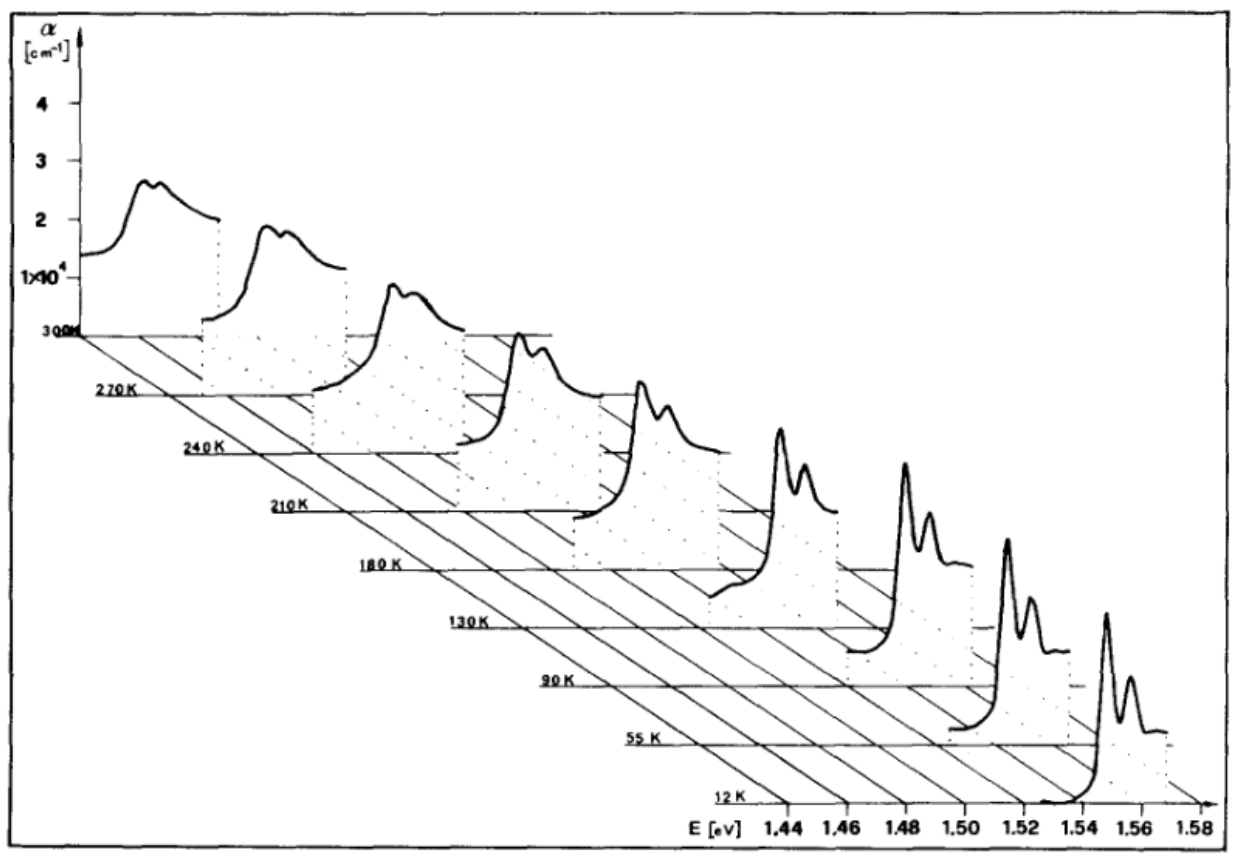
\includegraphics[scale=0.55]{images/chapter_optical_props/gaas_absorbance_filipowicz}
	\caption{GaAs/AlGaAs quantum well absorbance spectra at different temperatures. At higher temperatures, the presence of excitonic resonances is diminished. As the temperature decreases, two exciton peaks associated with light-hole and heavy-hole bands become more prominent. Reproduced from Ref.\ \cite{filipowicz1990temperature}.}
	\label{fig:gaas_vs_cnt_absorbance}
\end{figure}

%\subsection{The Effect of SWCNT Diameter}

%{\color{red} UNFINISHED}Curvature most directly refers to the diameter of the carbon nanotube \cite{blase1994hybridization}. It can influence the tendency of anti-bonding $\sigma^*$ and $\pi^*$ orbitals to hybridize, which can add further modifications to the band structure \cite{blase1994hybridization}. These effects are not fully accounted for in the zone-folding scheme.

%\begin{figure}[ht]
%	\centering
%	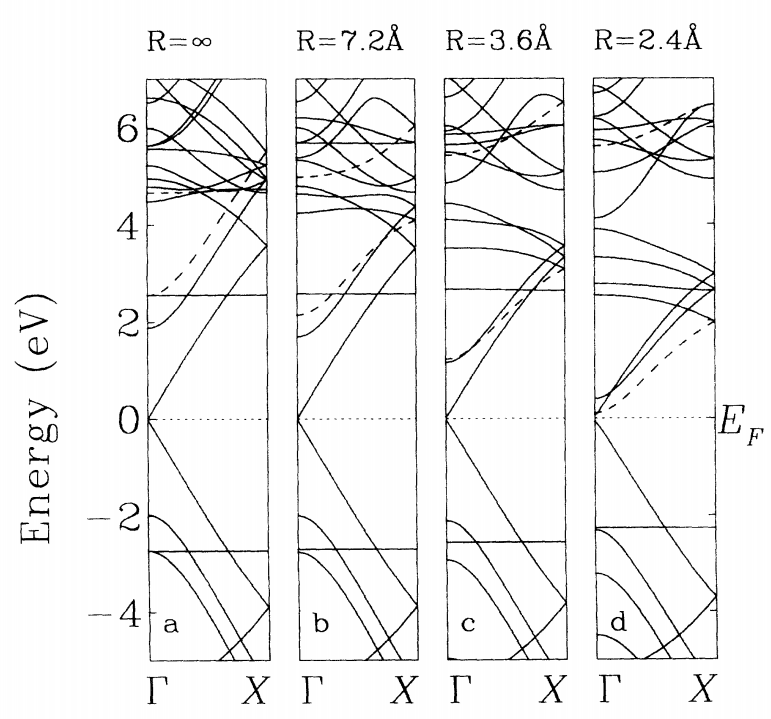
\includegraphics[scale=0.35]{images/chapter_optical_props/curvature_cnt_blase}
%	\caption{Tight-binding band structure of a (6,0) nanotube as a function of nanotube diameter $R$. The Fermi level remains at 0 eV. Moreover, the presence of $\sigma^*$ and $\pi^*$ hybridization, creates two new energy bands (dashed lines) that repel each other more strongly as the nanotube radius decreases. At the lowest radius, the low energy band gets very close to the valence band. However, ab-initio calculations reveal that this low energy branch actually intersects with the valence band. Reproduced from Ref.\ \cite{blase1994hybridization}.}
%	\label{fig:cnt_curvature}
%\end{figure}

%Figure \ref{fig:cnt_curvature} demonstrates this effect on the band structure of a (6,0) nanotube. The tight-binding model presented in the plots includes the effects of $\sigma^*$ and $\pi^*$ hybridization that manifest the presence of two new states whose difference in energy is determined by the nanotube diameter. At lower diameters, the lower energy band gradually gets closer to the valence band. In a full ab-initio calculation, this band would instead intersect with the conduction band to make the (6,0) nanotube have no band gap \cite{blase1994hybridization}. In contrast, a (9,0) nanotube that has a larger diameter would instead be predicted to have a narrow bandgap of 170 meV \cite{blase1994hybridization}.

\clearpage

\subsection{The Effect of External Dielectric Screening}

Coulomb interactions between carriers can become partially screened by the dielectric response of the medium in which CNTs are embeded \cite{ogawa1991optical}. These include electron-electron and electron-hole interactions that produce band gap renormalization ($E_\text{BGR}$) and determine the exciton binding energy ($E_\text{Bind}$) respectively, as shown in Figure \ref{fig:schematic_screening_walsh}. Given the extent at which Coulomb interactions have an impact on the optical properties of CNTs, it is clear that the screening of such interactions should affect the energies of optical transitions.

\begin{figure}[ht]
	\centering
	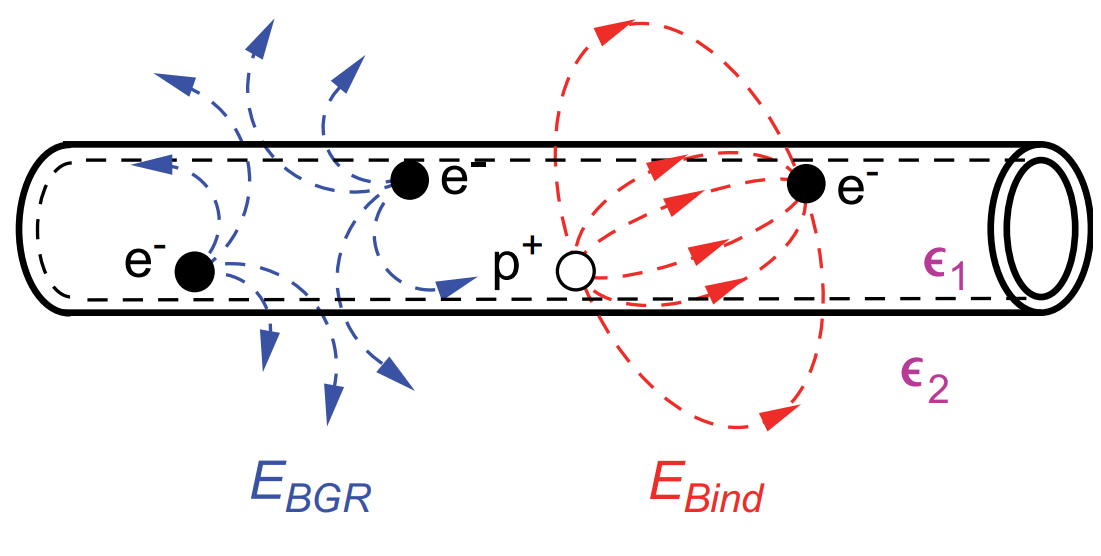
\includegraphics[scale=0.23]{images/chapter_optical_props/dielectric_screening_walsh_2007}
	\caption{Schematic diagram showing the two types of carrier-carrier interactions that influence the optical absorption spectrum. These include exciton binding ($E_\text{Bind}$) due to electron-hole interaction and band gap renormalization ($E_\text{BGR}$) caused by electron-electron interactions. Two relevant dielectric constants include $\epsilon_1$ and $\epsilon_2$ which represent the dielectrict constants of the CNT and the external environment respectively. In effect, the dielectric constant of the CNT environment can screen Coulomb interactions. Reproduced from \cite{walsh2008scaling}.}
	\label{fig:schematic_screening_walsh}
\end{figure}

Perebeinos \textit{et al}.\ (2004) studied this effect to determine how this dielectric screening affects the binding energy of excitons \cite{perebeinos2004scaling}. They ascertained that the exciton binding energy varies as $E_\text{b} \propto \epsilon^{-\alpha}$ for some constant $\alpha$ and a given dielectric constant $\epsilon$ \cite{perebeinos2004scaling}. However, they noted that the use of a single dielectric constant does not account for the fact that both the CNT itself as well as surrounding environment will contribute their own respective dielectric responses. Instead, this power law works well for narrow nanotubes embedded in environments with a dielectric constant much greater than that of the CNTs. Under these conditions the dielectric constant of the power law is given as that of the environment and the dielectric screening induced by the CNT itself is ignored. This description does not work well for environments where the dielectric constants of the CNT and the surrounding environment have relatively similar orders of magnitude.

Walsh \textit{et al}.\ (2007) extended this work by devising a model that accounts for both dielectric responses of CNTs and their surrounding environment. determined that $\alpha \approx 1.2$ \cite{walsh2008scaling}. In this work, they used an effective 1-D Coulomb potential $V_\text{1-D}^\text{Eff}(z)$ for an electron and a hole separated by a distance $z$. This potential was originally derived by Ogawa \textit{et al.} (1991) \cite{ogawa1991optical} and it accounts for the dielectric constant of the CNT, denoted as $\epsilon_1$, and the dielectric constant of the environment, written as $\epsilon_2$. Figure \ref{fig:coulomb_screening_walsh} shows a plot of how this 1-D potential how this potential becomes narrower due to screening for a fixed value of $\epsilon_1$ as $\epsilon_2$ increases. They determined that the exciton binding energy $E_\text{Bind}$ scales as
\begin{equation}
	E_\text{Bind} (\epsilon_2) = E_\text{Bind}^{\epsilon_2 = 1} / \epsilon_2^{1.2},
\end{equation}
where $ E_\text{Bind}^{\epsilon_2 = 1}$ represents the binding energy of a CNT suspended in air ($\epsilon_2 = 1$).

 \begin{figure}[ht]
 	\centering
 	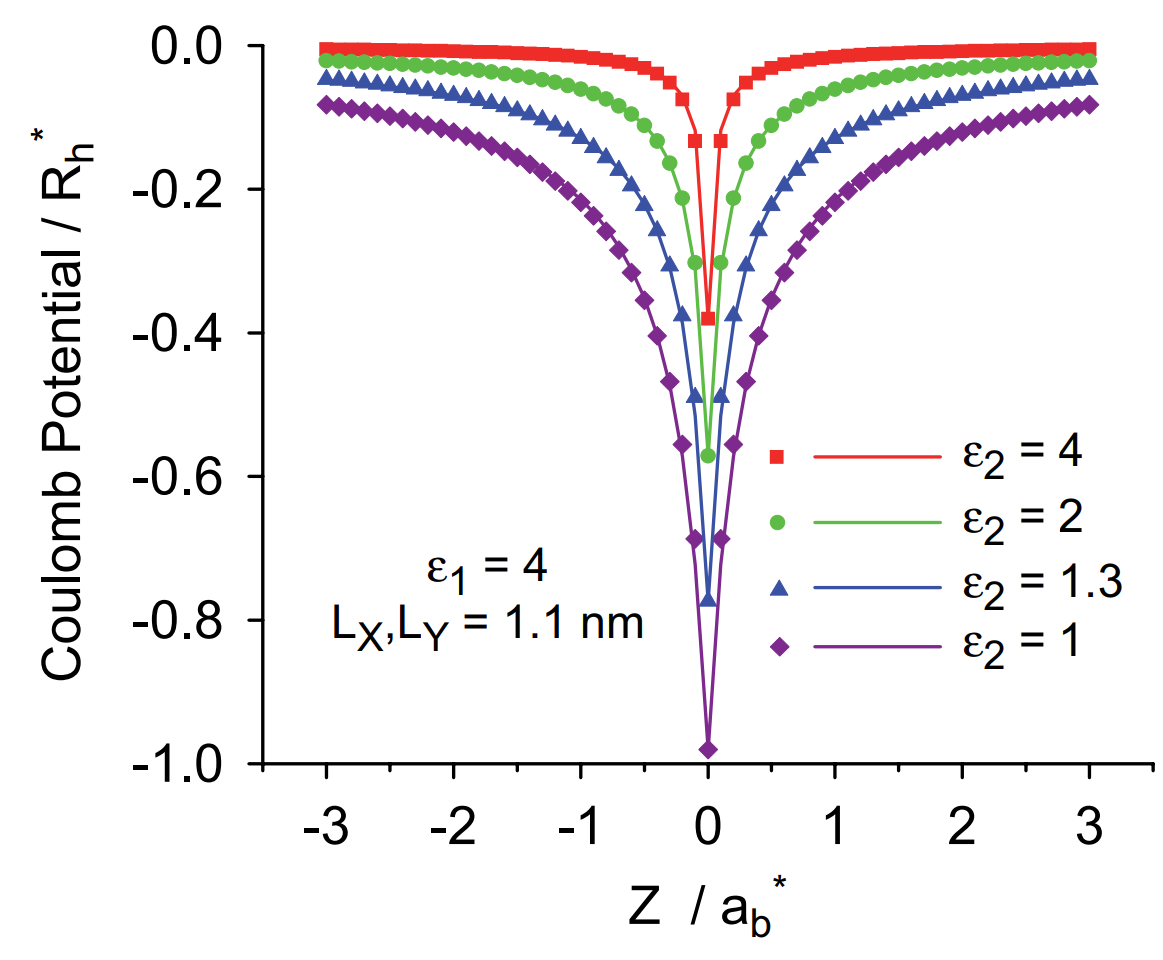
\includegraphics[scale=0.23]{images/chapter_optical_props/coulomb_potl_walsh}
 	\caption{ A 1-D Coulomb potential function between an electron and a hole separated by a distance $z$ plotted for different values of $\varepsilon_2$, the dielectric constant of the external evironment. Here, $\epsilon_1$ stands for the dielectric constant of the CNT. This function has been integrated over a CNT with lateral $x$ and $y$ lengths of 1.1 nm.  Here, $a_\text{b}^* = \epsilon_1 \hbar^2 / \mu e^2$ stands for the bulk exciton Bohr radius. As $\varepsilon_2$ increases, the potential function becomes spatially narrower due to the screening induced by the external environment. The potential function includes a cutoff parameter for $z$ to avoid the divergence as $z$ approaches zero. Reproduced from \cite{walsh2008scaling}.}
 	\label{fig:coulomb_screening_walsh}
 \end{figure}

In addition, they derived how the energies of optical resonances change with $\epsilon_2$. The optical transition energy $E_\text{OPT}$ depends on the total magnitude of band gap renormalization and the binding energy of excitons. This relationship can be expressed as%
%
\begin{equation}
	E_\text{OPT} = E_\text{SP} + E_\text{BGR} + E_\text{Bind},
\end{equation}
%
where $E_\text{SP}$ indicates the band gap energy that occurs when Coulomb interactions are neglected. In effect,  $E_\text{Opt}$ does not change very much as $ E_\text{BGR}$ and $E_\text{Bind}$ have opposite signs and relatively similar orders of magnitude. After accounting for effect of $\epsilon_2$, Walsh \textit{et al}.\ show that%
%
\begin{equation}
	E_\text{OPT}(\epsilon_2) = E_\text{SP} + E_\text{BGR}^{\epsilon_2 = 1}/\epsilon_2 + E_\text{Bind}^{\epsilon_2 = 1}/\epsilon_2^{1.2}.
\end{equation}
%
Figure \ref{fig:energy_shift_walsh} presents a plot of this expression. From previous mesurements of the $E_{22}$ transition, they determined the relevant paramters which include $E_\text{BGR}^{\epsilon_2 = 1} = 730$ meV and $E_\text{Bind}^{\epsilon_2 = 1} =$  580 meV \cite{walsh2007screening}. As the magnitude of $\epsilon_2$ increases, the optical resonance exhibits a very slight redshift.

\begin{figure}[ht]
	\centering
	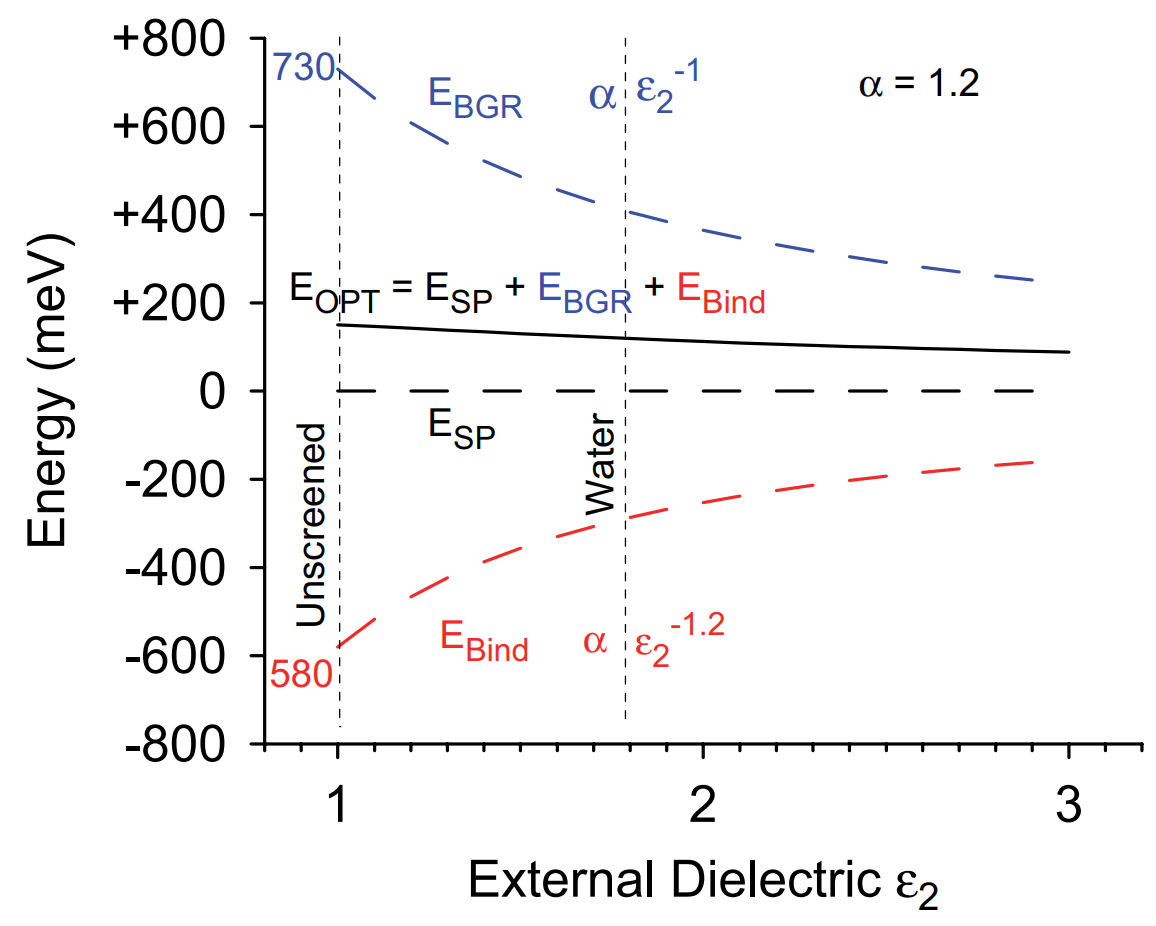
\includegraphics[scale=0.25]{images/chapter_optical_props/dielectric_binding_walsh_2007}
	\caption{ The effect of dielectric screening by the external environment on the energy of an optical resonance $E_\text{OPT}$. Here, $E_\text{SP}$ stands for the energy of the optical transition for a free electron when Coulomb interactions are ignored. Both band gap renormalization and the exciton binding energy have an effect on the energy of $E_\text{OPT}$. These two effects only cause a very marginal redshift of optical resonances as screening induced by the external environment increases. Reproduced from \cite{walsh2008scaling}.}
	\label{fig:energy_shift_walsh}
\end{figure}

These expectations have been verified through experiments conducted by Ohno \textit{et al.} (2007) \cite{ohno2007excitonic}. They measured $E_{11}$ and $E_{22}$ peak positions of an assortment of CNTs grown over trenches on a quartz substrate. By immersing the nanotubes in a variety of solvents with known dielectric constants, they measured the redshift of optical resonances as the dielectric constant of CNT environment increased. Figure \ref{fig:energy_shift_ohno} shows a summary of these results. Overall, the $E_{11}$ transitions redshifted by 33-49 meV whereas, the $E_{22}$ transition redshifted by 26-30 meV. These peak shifts began to saturate once the dielectric constant of the solvent became greater than 5.

\begin{figure}[ht]
	\centering
	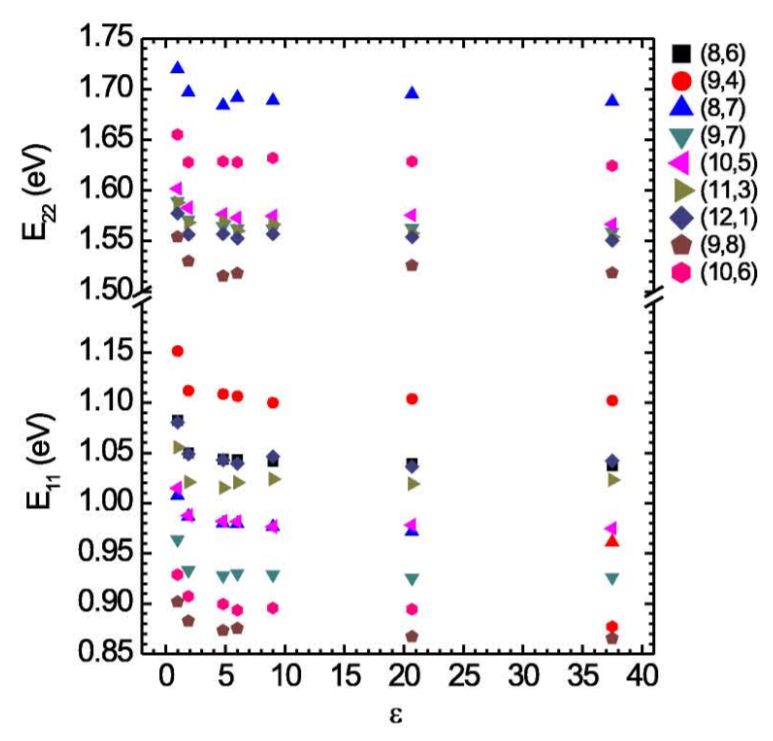
\includegraphics[scale=0.5]{images/chapter_optical_props/screening_ohno}
	\caption{Experimentally measured resonance energies for the $E_{11}$ and $E_{22}$ transitions occuring in various CNTs immersed in different dielectric environments. As the dielectric constant of the external envrionment increases, both optical resonances experience a slight redshift in energy. Reproduced from Ref.\ \cite{ohno2007excitonic}.}
	\label{fig:energy_shift_ohno}
\end{figure}

\clearpage

\subsection{Dark and Bright Excitons}

Theory suggests that each sub-band in the band structure of carbon nanotubes possesses up to 16 excitonic states \cite{amori2018excitons}. This determination takes into account the degeneracy of the $K$ and $K'$ points in the first Brillouin zone in graphene (4-fold degeneracy) as well as the spin-spin interactions of electron and hole carriers (4-fold degeneracy). In addition, short-range Coulomb interactions coming from inter-valley mixing and exchange interactions split these 16 possible excitonic states to give rise to a fine structure composed of 4 spin-singlet states and 12 spin-triplet states as shown in Figure \ref{fig:dark_bright_excitons_dispersion} \cite{ando2006effects}. Due to weak spin-orbit coupling, it is generally rare to convert a singlet state into a triplet state via phonon scattering processes \cite{amori2018excitons}.

Of the four singlet states, only one of these can be accessed via an optical transition and is therefore associated with every possible $E_\text{ij}$ resonance. This is commonly referred to as a ``bright" exciton state whereas, the remaining 3 singlet states are optically inactive meaning that they do not couple directly with light and are therefore said to be ``dark'' states.

\begin{figure}[ht]
	\centering
	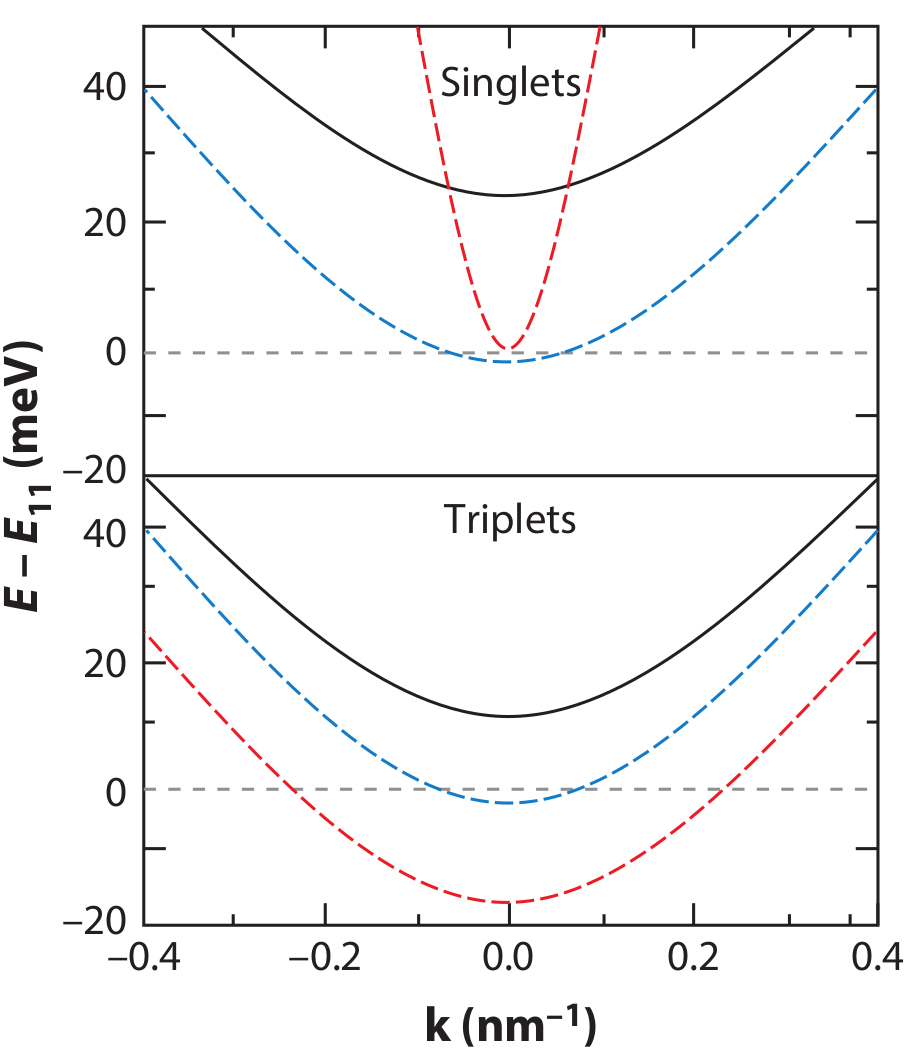
\includegraphics[scale=0.25]{images/chapter_optical_props/dark_and_bright_excitons}
	\caption{Energy dispersion of singlet and triplet states for a (19,0) nanotube. The black solid curves currespond to doubly-degenerate states with a non-zero angular momentum. The red dashed curves (second highest band for singlets, and lowest band for triplets) indicate odd-parity, bright states with zero angular momentum. Finally, the blue dashed curves (lowest band for singlets and second highest band for triplets) refer to even-parity, dark states. Reproduced from Ref.\ \cite{amori2018excitons}.}
	\label{fig:dark_bright_excitons_dispersion}
\end{figure}

Additionally, Figure \ref{fig:exciton_transitions} shows a schematic diagram describing the possible electron-hole configurations for singlet states. On one hand, the highest energy singlet states include charge carriers in the $K$ point bound to carriers in the $K'$ point, otherwise known as indirect excitons \cite{srivastava2008direct}. These states cannot be accessed by an optical transition as these transitions require the change in momentum between the initial and final states to be zero. On the other hand, the lowest energy singlet states, which include a bright and a dark state, refer to electrons and holes with the same momentum that are bound together \cite{srivastava2008direct}. The lowest energy singlet state is dipole-forbidden as a result of its even-parity. Despite this, it has been observed experimentally through a magnetic brightening process.

\begin{figure}[ht]
	\centering
	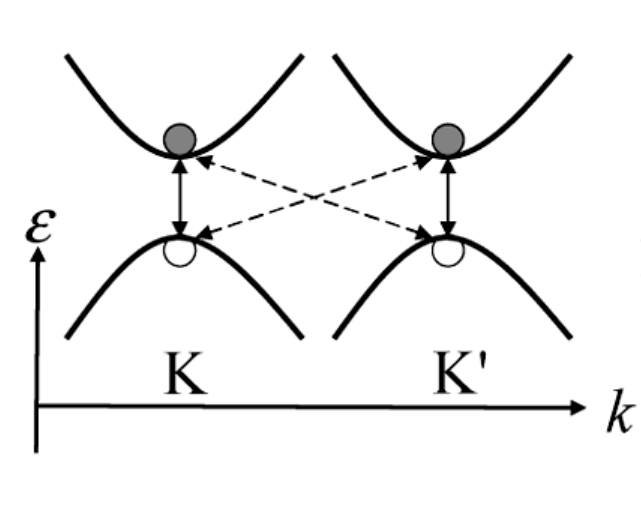
\includegraphics[scale=0.4]{images/chapter_optical_props/exciton_schematic_srivastava}
	\caption{Schematic energy dispersion for four possible spin-singlet exciton configurations. Two of these include indirect excitons appearing due to Coulomb interactions between carriers an electron (hole) in the $K$ point and a hole (electron) in the $K'$ point. The remaining two consist of excitons formed by electrons and holes with the same momentum. Reproduced from Ref.\ \cite{srivastava2008direct}.}
	\label{fig:exciton_transitions}
\end{figure}

The application of a magnetic field down the nanotube axis breaks time-reversal symmetry \cite{srivastava2008direct}. In a process known as the Aharonov-Bohm effect, the magnetic field lifts the degeneracy between $K$ and $K'$ states and brightens the dark singlet state closest in energy to the bright singlet state. Figure \ref{fig:exciton_brightening} shows the brightening of the dark exciton state in a series of magnetic field-dependent photoluminescence measurements on a single nanotube. With no magnetic field applied, the photoluminescence spectrum only contains emission from the bright exciton. At higher magnetic fields, a second lower energy peak emerges due to the brightening of the dark exciton state.

\begin{figure}[ht]
	\centering
	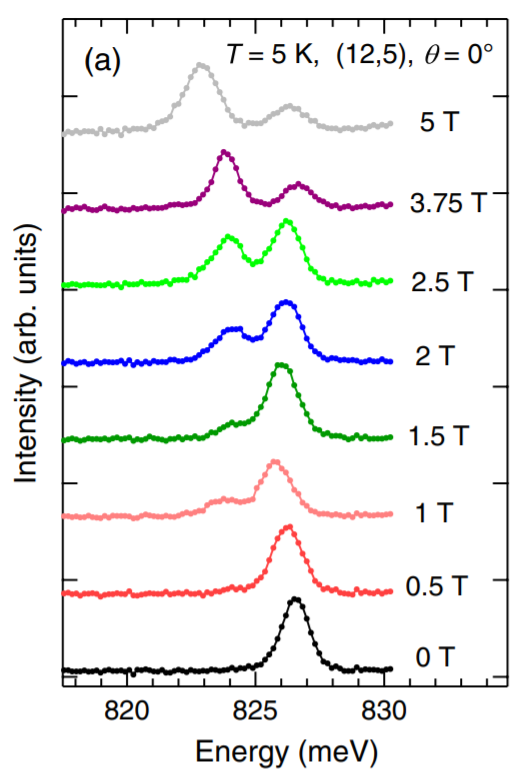
\includegraphics[scale=0.5]{images/chapter_optical_props/dark_brightening_srivastava}
	\caption{Magnetic-field dependent photoluminescence spectra obtained from a single carbon nanotube. The magnetic field is applied in a direction parallel to the nanotube axial direction. At 0 T, photoluminescnce only occurs due to the bright exciton state. At higher magnetic fields, a second emission peak appears due to the magnetic brightening of a dark exciton state as a result of the Aharonov-Bohm effect.  Reproduced from Ref.\ \cite{srivastava2008direct}.}
	\label{fig:exciton_brightening}
\end{figure}


%\subsection{Phonon Side-Bands}
%
%{\color{red} UNFINISHED} Exciton-phonon coupling \cite{perebeinos2005effect, yu2010phonon, plentz2005direct}. Absorption of light to form exciton-phonon bound state. In many nanotubes this state appears about 200 meV above the $E_{11}$ optical transition. Attributed to longitudinal optical phonon at the $K$ and $\Gamma$ points of the graphene Brillouin zone. Still conserve momentum light has negligible momentum, so we can get excitons with momentum $q$ and phonons with momentum $-q$. Suggests that exciton-phonon bound states may give indirect access to dark excitons.


\section{Summary}

Carbon nanotubes exhibit unique properties. They behave as either semiconducting or metallic materials depending on their chirality $(n,m)$. Furthermore, their 1-D character establishes anisotropic optical selection rules depending on the polarization of light with respect to the carbon nanotube axial direction. Moreover, the quantum confinement imposed by their 1-D structure enhances electron-electron interactions that mitigate the oscillator strength of free-electron states in the electronic band structure. These strong Coulomb interactions promote the presence of excitons with very high binding energies that are stable even at room temperatures, unlike those of conventional semiconductors. Indeed, two-photon measurements have corroborated this by revealing substantial evidence that all optical transitions in carbon nanotubes directly create excitons. Finally, of the 16 lowest-energy exciton states in SWCNTs, only one of these directly couples with light in each dipole-allowed transition.
